\باب{بکھراو}\شناخت{باب_بکھراو}
%typing complete
\حصہ{تعارف}
\جزوحصہ{کلاسیکی نظریہ بکھراو}
فرض کریں کسی مرکز بکھراو پر ایک ذرہ کا آمد ہوتا ہے مثلاً ایک پروٹان کو ایک بھاری مرکزہ پر داغا جاتا ہے یہ توانائی \عددی{E}  اور ٹکراو مقدار معلوم \عددی{b} کے ساتھ آ کر کسی زاویہ  بکھراو \عددی{\theta} پر اُبھرتا ہے  ؛ شکل \حوالہ{شکل_بکھراو_کلاسیکی_ٹکراو_اور_زاویہ}  دیکھیں۔ میں اپنی آسانی کے لئے فرض کرتا ہوں کہ ہدف اسمتی تشاکلی ہے یوں خط حرکت ایک مستوی میں پایا جائے گا اور کہ نشانہ بھاری ہے لہٰذا  تصادم  کی بنا پر اس کی اچھال  کو نظرانداز کیا جا سکتا ہے۔ کلاسیکی نظریہ بکھراو کا بنیادی مسئلہ یہ ہوگا: ٹکراو مقدار معلوم کو جانتے ہوئے زاویہ بکھراو کا حساب کریں۔ یقیناً عام طور پر ٹکراو مقدار معلوم جتنا چھوٹا ہو زاویہ بکھراو اتنا بڑا ہوگا۔
\begin{figure}
\centering
\begin{tikzpicture}[]
\draw[-stealth] (0,0) -- (5,0) node[below]{$z$};
\draw[dashed] (0,0.5) -- (5,0.5);
\draw[thick,->-=0.5] (0,0.5) to [out=0,in=-120] (5,4);
\draw[dashed] (3.25,0.5) -- (5,4);
\draw[]([shift={(0:0.5)}]3.25,0.5) arc (0:60:0.5) node[pos=0.5,right]{$\theta$};
\draw[stealth-stealth] (0.4,0) -- (0.4,0.5) node[pos=0.5,left]{$b$};
\draw[] (3.5,0) node[circle,inner sep= 1.5pt,fill=black]{} node[below]{\RL{نقطہ بکھراو}};
\end{tikzpicture}
\caption{کلاسیکی مسئلہ بکھراو، جس میں ٹکراو مقدار معلوم \عددی{b} اور زاویہ بکھراو \عددی{\theta} کی وضاحت کی گئی ہے۔}
\label{شکل_بکھراو_کلاسیکی_ٹکراو_اور_زاویہ}
\end{figure}


\ابتدا{مثال}
\موٹا{سخت کرہ کا بکھراو}۔ فرض کریں ہدف رداس \عددی{R} کا ایک ٹھوس بھاری گیند ہے جبکہ آمدی ذرہ ہوائی بندوق کا ایک چھرا  ہے جو لچھکیلی ٹپکی کھا کر مڑتا ہے  (شکل \حوالہ{شکل_بکھراو_سخت_کرہ_لچکدار})۔ زاویہ \عددی{\ایلفا} کی صورت میں ٹکراو مقدار معلوم \عددی{b=R\sin\ایلفا} اور زاویہ بکھراو \عددی{\تھیٹا=\پاے-2\ایلفا} ہوں گے۔ یوں درج ذیل ہوگا۔
\begin{align}
	b = R\sin\left(\frac{\pi}{2}-\frac{\theta}{2}\right) = R\cos\left(\frac{\theta}{2}\right)
\end{align}

\begin{figure}
\centering
\pgfmathsetmacro{\r}{1.5}
\pgfmathsetmacro{\ang}{35}
\pgfmathsetmacro{\b}{\r*sin(\ang)}
\pgfmathsetmacro{\c}{\r*cos(\ang)}
\begin{tikzpicture}[]
\draw[] (0,0) node[circle, inner sep=1.5pt, fill=black]{} circle (\r);
\draw[-stealth] (-5,0) -- (2,0) node[below]{$z$};
\draw[stealth-stealth] (-4.4,0) --++ (0,\b) node[pos=0.5,left]{$b$};
\draw[thick,-stealth] (-5,\b) -- (-\c,\b) --++ (180-2*\ang:2);
\draw[dashed] (-\c, \b) --++ (1.25,0);
\draw[dashed] (0,0) --++ (180-\ang:3) node[pos=0.25,shift={(90-\ang:0.75em)}]{$R$};
\draw[] ([shift={(180-\ang:0.5)}]0,0) arc (180-\ang:180:0.5) node[pos=0.4,left]{$\alpha$};
\draw[] ([shift={(180-\ang:0.5)}]-\c,\b) arc (180-\ang:180:0.5) node[pos=0.4,left]{$\alpha$};
\draw[] ([shift={(180-2*\ang:0.4)}]-\c,\b) arc (180-2*\ang:180-\ang:0.4) node[pos=0.5,shift={(180-1.5*\ang:0.75em)}]{$\alpha$};
\draw[] ([shift={(0:0.75)}]-\c,\b) arc (0:180-2*\ang:0.75) node[pos=0.5,above]{$\theta$};
\end{tikzpicture}
\caption{سخت کرہ سے لچکدار بکھراو۔}
\label{شکل_بکھراو_سخت_کرہ_لچکدار}
\end{figure}

ظاہری طور پر درج ذیل ہوگا
\begin{align}
	\theta =
	\begin{cases}
		2\cos^{-1}(b/R), & b\leq R \text{\RL{اگر}} \\
		0, & b\geq R \text{\RL{اگر}}
	\end{cases}
\end{align}
\انتہا{مثال}
%=================================
\begin{figure}
\centering
\pgfmathsetmacro{\r}{2}
\pgfmathsetmacro{\ta}{30}
\pgfmathsetmacro{\tb}{40}
\pgfmathsetmacro{\pa}{40}
\pgfmathsetmacro{\pb}{80}
\pgfmathsetmacro{\ia}{0.5}
\pgfmathsetmacro{\ib}{0.3}
\pgfmathsetmacro{\tcc}{\ta+(\tb-\ta)/2}
\pgfmathsetmacro{\tdd}{\pa+(\pb-\pa)/2}
\begin{tikzpicture}[declare function={fa(\t,\p)=\r*sin(\t)*cos(\p);fb(\t,\p)=\r*sin(\t)*sin(\p);fc(\t,\p)=\r*cos(\t);}, 
x={(0cm,-0.25cm)}, y={(1cm,0cm)}, z={(0cm,1cm)}]
\begin{scope}[rotate=-90]
\draw[] plot [domain=0:360,smooth]({fa(\x,90)},{fb(\x,90)},{fc(\x,90)});
\draw[] plot [domain=-90:90,smooth]({fa(\ta,\x)},{fb(\ta,\x)},{fc(\ta,\x)});
\draw[] plot [domain=-90:90,smooth]({fa(\tb,\x)},{fb(\tb,\x)},{fc(\tb,\x)});
%\draw[dashed] plot [domain=90:270]({fa(\ta,\x)},{fb(\ta,\x)},{fc(\ta,\x)});
%\draw[dashed] plot [domain=90:270]({fa(\tb,\x)},{fb(\tb,\x)},{fc(\tb,\x)});
\draw[] plot [domain=\ta:\tb]({fa(\x,\pa)},{fb(\x,\pa)},{fc(\x,\pa)});
\draw[] plot [domain=\ta:\tb]({fa(\x,\pb)},{fb(\x,\pb)},{fc(\x,\pb)});
\coordinate (tta) at ({fa(\ta,\pa)},{fb(\ta,\pa)},{fc(\ta,\pa)});
\coordinate (ttb) at ({fa(\ta,\pb)},{fb(\ta,\pb)},{fc(\ta,\pb)});
\coordinate (ppa) at ({fa(\tb,\pa)},{fb(\tb,\pa)},{fc(\tb,\pa)});
\coordinate (ppb) at ({fa(\tb,\pb)},{fb(\tb,\pb)},{fc(\tb,\pb)});
\draw[] (tta) -- (0,0,0);
\draw[] (ttb) -- (0,0,0);
\draw[] (ppa) -- (0,0,0);
\draw[] (ppb) -- (0,0,0);
\draw[] (0,0,0) node[circle,inner sep=1.5pt,fill=black]{} -- ({fa(\ta,-90)},{fb(\ta,-90)},{fc(\ta,-90)});
\draw[] (0,0,0) -- ({fa(\tb,-90)},{fb(\tb,-90)},{fc(\tb,-90)});
\draw[] (0,0,-6) -- (0,0,2.5);
\draw[] plot [domain=0:\ta] ({0.4*fa(\x,-90)},{0.4*fb(\x,-90)},{0.4*fc(\x,-90)});
\draw[] ({0.4*fa(\ta/2,-90)},{0.4*fb(\ta/2,-90)},{0.4*fc(\ta/2,-90)}) node[right,yshift=0.25em]{$\theta$};
\draw[] plot [domain=\ta:\tb]({0.5*fa(\x,-90)},{0.5*fb(\x,-90)},{0.5*fc(\x,-90)});
\draw[] ({0.5*fa(\ta,-90)},{0.5*fb(\ta,-90)},{0.5*fc(\ta,-90)}) node[pin={[]160:{$\dif\theta$}}]{};
\draw[] plot [domain=0:360] ({\ia*fa(90,\x)},{\ia*fb(90,\x)},{-5+\ia*fc(90,\x)});
\draw[] plot [domain=0:360] ({\ib*fa(90,\x)},{\ib*fb(90,\x)},{-5+\ib*fc(90,\x)});
\coordinate (iia) at ({\ia*fa(90,\pa)},{\ia*fb(90,\pa)},{-5+\ia*fc(90,\pa)});
\coordinate (iib) at ({\ib*fa(90,\pa)},{\ib*fb(90,\pa)},{-5+\ib*fc(90,\pa)});
\coordinate (iic) at ({\ia*fa(90,\pb)},{\ia*fb(90,\pb)},{-5+\ia*fc(90,\pb)});
\coordinate (iid) at ({\ib*fa(90,\pb)},{\ib*fb(90,\pb)},{-5+\ib*fc(90,\pb)});
\draw[] (iia) -- (iib);
\draw[] (iic) -- (iid);
\path[name path=za] plot [domain=\pa:\pb] ({\ia*fa(90,\x)},{\ia*fb(90,\x)},{-5+\ia*fc(90,\x)});
\path[name path=zb] plot [domain=\pa:\pb] ({\ib*fa(90,\x)},{\ib*fb(90,\x)},{-5+\ib*fc(90,\x)});
\tikzfillbetween[of=za and zb]{gray,opacity=0.5};
\path[name path=zc] plot [domain=\pa:\pb,smooth]({fa(\ta,\x)},{fb(\ta,\x)},{fc(\ta,\x)});
\path[name path=zd] plot [domain=\pa:\pb,smooth]({fa(\tb,\x)},{fb(\tb,\x)},{fc(\tb,\x)});
\tikzfillbetween[of=zc and zd]{gray,opacity=0.5};
\draw[thick] ($(iia)!0.5!(iid)$) coordinate(bba) --++ (0,0,-1) coordinate(bbb);
\draw[thick] ($(iia)!0.5!(iid)$) --++ (0,0,4.5) coordinate(kleft);
\draw[line width=2pt,-stealth,white] ($(tta)!0.5!(ppb)$) coordinate(kright) --({1.75*fa(\tcc,\tdd)},{1.75*fb(\tcc,\tdd)},{1.75*fc(\tcc,\tdd)});
\draw[thick,-stealth] ($(tta)!0.5!(ppb)$) coordinate(kright) --({1.75*fa(\tcc,\tdd)},{1.75*fb(\tcc,\tdd)},{1.75*fc(\tcc,\tdd)});
\draw[thick] (kleft) to [out=90,in=245] (kright);
\draw[stealth-,shorten <=1.5pt] ($(iia)!0.5!(iic)$) --++ (0.5,0.5) node[below]{$\dif\sigma$};
\draw[stealth-stealth] (0,0,-5.75) -- ($(bba)!(0,0,-5.75)!(bbb)$) node[pos=0.5,left]{$b$};
\draw[] (iib) -- (0,0,-5);
\draw[] (iid) -- (0,0,-5);
\path[]($(iia)!0.5!(iid)$)--(0,0,-5)coordinate[pos=0.5](kkphi);
\draw[] (kkphi) to [out=90,in=-90] ++ (0,-1,1)node[right]{$\dif \phi$};
\draw[] plot [domain=\ta-15:\tb+7] ({0.3*fa(\x,90)},{0.3*fb(\x,90)},{0.3*fc(\x,90)});
\draw[] plot [domain=\ta-15:\tb+7] ({0.35*fa(\x,90)},{0.35*fb(\x,90)},{0.35*fc(\x,90)});
\draw[]({0.35*fa(\tcc,90)},{0.35*fb(\tcc,90)},{0.35*fc(\tcc,90)})--++(0,0.75,0.3)node[below]{$\dif\Omega$};
\end{scope}
\end{tikzpicture}
\caption{رقبہ \عددی{\dif \sigma} میں آمدی ذرات ٹھوس زاویہ \عددی{\dif\Omega} میں بکھرتے ہیں۔}
\label{شکل_بکھراو_آمدی_اور_ٹھوس_زاویہ}
\end{figure}



عمومی طور پر لامتناہی چھوٹے رقبہ عمودی تراش \عددی{\dif\سگما} میں آمدی ذرات مطابقتی لامتناہی چھوٹے
 ٹھوس زاویہ \عددی{\dif\بڑااومیگا} میں بکھریں گے (شکل \حوالہ{شکل_بکھراو_آمدی_اور_ٹھوس_زاویہ})۔ بڑی \عددی{\dif\سگما} کی صورت میں \عددی{\dif\بڑااومیگا} بھی بڑا ہوگا تناسبی جزو ضربی \عددی{D(\تھیٹا)\equiv\dif\سگما/\dif\بڑااومیگا} کو تفریقی بکھراو عمودی تراش کہتے ہیں 
\begin{align}
	\dif\sigma = D(\theta)\dif\Omega
\end{align}
ٹکراو مقدار معلوم اور اسمتی زاویہ \عددی{\فاے} کی صورت میں \عددی{\dif\سگما=b\dif b\dif\فاے} اور \عددی{\dif\بڑااومیگا=\sin\تھیٹا\dif\تھیٹا\dif\فاے} ہوں گے لہٰذا درج ذیل ہوگا
\begin{align}
	D(\theta) = \frac{b}{\sin\theta}\abs{\frac{\dif b}{\dif\theta}}
\end{align}
چونکہ عمومی طور پر \عددی{\تھیٹا} مقدار معلوم \عددی{b} کا گھٹتا ہوا تفاعل ہوگا لہٰذا یہ تفرق در حقیقت منفی ہوگا اسی لئے مطلق قیمت لی گئی ہے۔

\ابتدا{مثال}
\موٹا{سخت کرہ کے بکھراو کی مثال جاری رکھتے ہیں}۔ سخت کرہ بکھراو \حوالہء{مثال \num{11.1}} کی صورت میں 
\begin{align}
	\frac{\dif b}{\dif\theta}=-\frac{1}{2}R\sin\left(\frac{\theta}{2}\right)
\end{align}
لہٰذا درج ذیل ہوگا 
\begin{align}
	D(\theta) = \frac{R\cos(\theta/2)}{\sin\theta}\left(\frac{R\sin(\theta/2)}{2}\right) = \frac{R^2}{4}
\end{align}
اس مثال میں تفریقی عمودی تراش \عددی{\تھیٹا} کا تابع نہیں ہے جو ایک غیر معمولی بات ہے۔
\انتہا{مثال}
کل عمودی تراش تمام ٹھوس زاویوں پر \عددی{D(\تھیٹا)} کا تکمل ہوگا
\begin{align}
	\sigma\equiv\int D(\theta)\dif\Omega	
\end{align}
اندازاً بات کرتے ہوئے یہ آمدی شعاع کا وہ رقبہ ہوگا جسے ہدف بکھیرتا ہے۔ مثال کے طور پر سخت کرہ بکھراو کی صورت میں درج ذیل ہوگا
\begin{align}
	\sigma = (R^2/4)\int \dif\Omega = \pi R^2
\end{align}
جو ہمارے توقعات کے عین مطابق ہے۔ یہ کرہ کا رقبہ عمودی تراش ہے۔ اس رقبہ میں آمدی چھرے  ہدف کو نشانہ بنائیں گے جبکہ اس سے باہر چھرے ہدف کو خطا کریں گے۔ یہی تصورات نرم اہداف مثلاً مرکزہ کا کولمب میدان کے لئے بھی کار آمد ہے جن میں صرف نشانے پر لگنا یا نہ لگنا نہیں ہوگا۔

آخر میں فرض کریں ہمارے پاس آمدی ذرات کی یکساں شدت تابندگی کی ایک شعاع ہو 
\begin{align}
	\mathcal{L}\equiv\text{\RL{اکائی رقبہ پر فی اکائی وقت آمدی ذرات کی تعداد}}
\end{align}
فی اکائی وقت رقبہ \عددی{\dif\سگما} میں داخل ہونے والے ذرات اور یوں ٹھوس زاویہ \عددی{\dif\بڑااومیگا} میں بکھراو والے ذرات کی تعداد \عددی{\dif N = \mathcal{L}\dif\سگما=\mathcal{L}D(\تھیٹا)\dif\بڑااومیگا}  ہوگی لہٰذا درج ذیل ہوگا 

\begin{align}
	D(\theta) = \frac{1}{\mathcal{L}}\frac{\dif N}{\dif\Omega}
\end{align}
چونکہ یہ صرف ان مقداروں کی بات کرتا ہے جنہیں تجربہ گاہ میں با آسانی ناپا جا سکتا ہو لہٰذا اس کو عموماً تفریقی عمودی تراش کی تعریف لیا جاتا ہے۔ اگر ٹھوس زاویہ \عددی{\dif\بڑااومیگا} میں بکھرے ذرات کو محسوس کار دیکھتا ہو تب ہم اکائی وقت میں معلوم شدہ ذرات کی تعداد کو \عددی{\dif\بڑااومیگا} سے تقسیم کر کے آمدی شعاع کی تابندگی کے لحاظ سے معمول شدہ کرتے ہیں۔

\ابتدا{سوال}
\موٹا{ردرفورڈ بکھراو}۔ بار \عددی{q_1} اور حرکی توانائی \عددی{E} کا ایک آمدی ذرہ ایک بھاری ساکن ذرہ جس کا بار \عددی{q_2} ہو 	سے بکھرتا ہے۔

(الف) ٹکراو مقدار معلوم اور زاویہ بکھراو کے بیچ رشتہ اغز کریں۔

جواب: \عددی{b=(q_1q_2/8\pi\epsilon_0E)\cot(\theta/2)}

(ب) تفریقی بکھراو عمودی تراش تعین کریں۔

جواب:
\begin{align}
	D(\theta)=\left[\frac{q_1q_2}{16\pi\epsilon_0E\sin^2(\theta/2)}\right]^2
\end{align}
(ج) دکھائیں کہ ردرفورڈ بکھراو کا کل عمودی تراش لامتناہی ہوگا۔ ہم کہتے ہیں \عددی{1/r} مخفیہ لامتناہی ساتھ رکھتا ہے آپ کولمب قوت سے بچ نہیں سکتے ہیں۔
\انتہا{سوال}
%==========================

\جزوحصہ{کوانٹائی نظریہ بکھراو}
بکھراو کے کوانٹائی نظریہ میں فرض کرتے ہیں کہ ایک آمدی مستوی موج \عددی{\psi(z) = Ae^{ikz}} جو محور \عددی{z} رخ حرکت کرتی ہو کا سامنا ایک بکھراو مخفیہ سے ہوتا ہے جس کے نتیجہ میں ایک کروی رخصتی موج پیدا ہوتی ہے  (شکل \حوالہ{شکل_بکھراو_مستوی_آمدی_کروی_رخصتی})۔   یعنی ہم مساوات شروڈنگر کے وہ حل تلاش کرنا چاہتے ہیں جن کی عمومی روپ درج ذیل ہو
\begin{align}
	\psi(r, \theta)\approx A\left\{e^{ikz}+f(\theta)\frac{e^{ikr}}{r}\right\}, && \text{\RL{کے لئے}} r \text{\RL{بڑے}}
\end{align}
%
\begin{figure}
\centering
\pgfmathsetmacro{\r}{0.5}
\pgfmathsetmacro{\anga}{35}
\pgfmathsetmacro{\angb}{110}
\pgfmathsetmacro{\angc}{10}
\pgfmathsetmacro{\a}{\r/3}
\begin{tikzpicture}
\draw[-stealth] (-6,0) -- (2.75,0) node[below]{$z$};
\foreach \n in {1,2,3,4}{\draw (0,0) circle (\n*\r);}
\draw[fill=black] (0,0) circle (1.5pt);
\draw[] (0,0) circle (3.5pt);
\draw[] (0,0) --++ (\anga:2.5);
\draw[] (0,0) ++ (\angb:1.5*\r) ++ (\angb-90:\a) --++ (\angb-\angc:3*\r) --++ (\angb-90:\r/2) coordinate(za);
\draw[] (0,0) ++ (\angb:1.5*\r) ++ (\angb+90:\a) --++ (\angb+\angc:3*\r) --++ (\angb+90:\r/2) coordinate(zb);
\draw[] (\angb:5.5*\r) -- (za) node[right]{$e^{ikr}$};
\draw[] (\angb:5.5*\r) -- (zb);
\draw[] (\anga/2:1.5*\r) node[]{$\theta$};
\foreach \n in {1,2,3,4,5} {\draw[] (-3-\n*\r,1.5) --++ (0,-3);}
\draw[] (-3-2.5*\r,-\r) --++ (2.5*\r,0) --++ (0,0.25*\r) coordinate(zc);
\draw[] (-3-2.5*\r,-1.5*\r) --++ (2.5*\r,0) --++ (0,-0.25*\r) coordinate(zd);
\draw[] (-3-2.5*\r,-1.25*\r) ++ (3*\r,0) coordinate(ze);
\draw[] (zc) -- (ze);
\draw[] (zd) -- (ze); 
\draw[] (-3-3*\r,-1.5) node[below]{$e^{ikz}$};
\end{tikzpicture}
\caption{	امواج کا بکھراو؛ آمدی مستوی موج    رخصتی کروی موج پیدا کرتی ہے۔}
\label{شکل_بکھراو_مستوی_آمدی_کروی_رخصتی}
\end{figure}

کروی موج میں جزو ضربی \عددی{1/r} پایا جاتا ہے چونکہ احتمال کی بقا کے خاطر \عددی{\abs{\psi}^2} کا یہ حصہ \عددی{1/r^2} کے لحاظ سے تبدیل ہوگا۔ عدد موج \عددی{k} کا آمدی ذرات کی توانائی کے ساتھ ہمیشہ کی طرح درج ذیل رشتہ ہوگا 
\begin{align}
	k\equiv\frac{\sqrt{2mE}}{\hslash}
\end{align}
یہاں بھی میں فرض کرتا ہوں کہ ہدف اسمتی تشاکلی ہے زیادہ عمومی صورت میں رخصتی کروی موج کا حیطہ \عددی{f} متغیرات \عددی{\فاے} اور \عددی{\تھیٹا} کا تابع ہوگا۔
\begin{figure}
\centering
\pgfmathsetmacro{\ra}{1.5}
\pgfmathsetmacro{\rb}{1}
\pgfmathsetmacro{\anga}{70}
\pgfmathsetmacro{\angb}{-30}
\pgfmathsetmacro{\d}{3}
\pgfmathsetmacro{\angc}{(\anga+\angb)/2}
\pgfmathsetmacro{\rc}{(\ra+\rb)/2}
\begin{tikzpicture}
\draw[fill=lgray,opacity=0.5] ([shift={(\angb:\ra)}]0,0) arc (\angb:\anga:\ra) coordinate(za)coordinate[pos=0](zaa)--(\anga:\rb) 
([shift={(\anga:\rb)}]0,0) arc (\anga:\angb:\rb) coordinate(zbb)coordinate[pos=0](zb)--(\angb:\ra);

\draw[] ([shift={(\angb:\ra)}]\d,0) arc (\angb:\anga:\ra) coordinate(zc)coordinate[pos=0](zcc);
\draw[dashed] ([shift={(\angb:\rb)}]\d,0) arc (\angb:\anga:\rb) coordinate(zd)coordinate[pos=0](zdd);
\draw[dashed] (zc) -- (zd);
\draw[dashed] (zcc) -- (zdd);
\draw(za)--(zc);
\draw(zaa)--(zcc);
\draw[dashed](zb)--(zd);
\draw[dashed](zbb)--(zdd);
\draw[decorate,decoration={brace,amplitude=5pt,raise=4pt,mirror}] (zaa)--(zcc) node[pos=0.5,yshift=-1.5em]{$v\dif t$};
\draw[] (\angc:\rc) node[pin={-135:{$\dif \sigma$}}]{};
\draw[-stealth] (\angc:\rc) ++ (\d+0.5,0) --++ (1.5,0) node[pos=0.5,above]{$v$};
\end{tikzpicture}
\caption{وقت \عددی{\dif t} کے دوران رقبہ \عددی{\dif\sigma} سے گزرتی  ہوئی آمدی  شعاع کا حجم \عددی{\dif V} ہے۔}
\label{شکل_بکھراو_رقبہ_حجم_شعاع}
\end{figure}



ہمیں حیطہ بکھراو \عددی{f(\تھیٹا)} تعین کرنا  ہوگا۔ یہ ہمیں کسی مخصوص رخ \عددی{\تھیٹا} میں بکھراو کا احتمال دیتا ہے اور یوں اس کا تعلق تفریقی عمودی تراش سے ہوگا۔ یقیناً سمتی رفتار \عددی{v} پر چلتے ہوئے ایک آمدی ذرہ کا وقت \عددی{\dif t} میں لامتناہی چھوٹی رقبہ \عددی{\dif\سگما} میں سے گزرنے کا احتمال   (شکل \حوالہ{شکل_بکھراو_رقبہ_حجم_شعاع}  دیکھیں)  درج ذیل ہوگا
\begin{align*}
	\dif P = \abs{\psi_{\text{\RL{آمدی}}}}^2\dif V = \abs{A}^2(v\dif t)\dif\sigma
\end{align*}
لیکن مطابقتی ٹھوس زاویہ \عددی{\dif\Omega} میں اس ذرہ کے بکھراو کا احتمال 
\begin{align*}
	\dif P = \abs{\psi_{\text{\RL{بکھرا}}}}^2\dif V = \frac{\abs{A}^2\abs{f}^2}{r^2}(v\dif t)r^2\dif\Omega
\end{align*}
بھی یہی ہوگا لہٰذا \عددی{\dif\sigma=\abs{f}^2\dif\Omega} اور درج ذیل ہوں گے
\begin{align}
		D(\theta) = \frac{\dif\sigma}{\dif\Omega} = \abs{f(\theta)}^2
\end{align}
ظاہر ہے کہ تفرقی عمودی تراش جس میں تجربہ کرنے والا دلچسپی رکھتا ہے حیطہ بکھراو جو مساوات شروڈنگر کے حل سے حاصل ہوگا کی مطلق مربع کے برابر ہوگا آنے والے حصوں میں ہم حیطہ بکھراو کی حساب کے دو تراکیب جزوی موج تجزیہ اور بارن تخمین پر غور کریں گے۔

\ابتدا{سوال}
ایک بُعدی اور دو ابعادی بکھراو کے لئے \حوالہء{مساوات \num{11.12}} کے مماثل تیار کریں۔
\انتہا{سوال} 



%=======================
% section 11.2 to end of chapter. unedited

\حصہ{جزوی موج تجزیہ}
\جزوحصہ{اصول و ضوابط}
ہم نے باب 4 میں دیکھا کہ کروی تشاکلی مخفیہ \عددی{V(r)} کے لئے مساوات شروڈنگر قابلِ علیحدگی حلوں
\begin{align}
	\psi(r, \theta, \phi) = R(r)Y^m_{\ell}(\theta, \phi)
\end{align}
کا حامل ہوگا جہاں \(Y_{\ell}^m\) کروی ہارمونی مساوات \num{4.32} ہے اور \(u(r) = rR(r)\) رداسی مساوات مساوات \num{4.37} 
\begin{align}
	-\frac{\hbar^2}{2m}\frac{d^2u}{dr^2}+\left[V(r)+\frac{\hbar^2}{2m}\frac{\ell(\ell+1)}{r^2}\right]u = Eu
\end{align}
کو مطمئن  کرتا ہے بہت بڑی \عددی{r} کی صورت میں مخفیہ صفر کو پہنچتا ہے اور مرکز گریز حصہ قابل نظرانداز ہوگا۔ لہٰذا درج ذیل لکھا جا سکتا ہے۔
\begin{align*}
	\frac{d^2u}{dr^2} \approx-k^2u
\end{align*}
اس کا عمومی حل درج ذیل ہے
\begin{align*}
	u(r) = Ce^{ikr}+De^{-ikr}
\end{align*}
پہلا جزو  رخصتی کروی موج کو اور دوسرا جزو  آمدی موج کو ظاہر کرتا ہے پھر ہے کہ موج  بکھراو کے لئے ہم \(D=0\) چاہتے ہیں۔ یوں بہت بڑی \عددی{r} کی صورت میں درج ذیل ہوگا
\begin{align*}
	R(r)\sim\frac{e^{ikr}}{r}
\end{align*}
جہاں ہم گزشتہ حصہ میں طبیعی وجوہات سے آغاز کر چکے ہیں مساوات  \num{11.12}۔

\begin{figure}
\centering
\begin{tikzpicture}
\draw[] (0,0) node[]{$V=0$} circle (0.6);
\draw[] (0,0) node[]{$V=0$} circle (2);
\draw[stealth-] (-160:0.6) to [out=-160,in=0] ++ (-1.5,-0.75) node[left]{\RL{خطہ بکھراو}};
\draw[] (0,1) node[yshift=-0.25em]{$V\equiv 0$} node[above]{\RL{درمیانہ خطہ}};
\draw[] (3,0.5) node[]{\RL{اشعاعی خطہ}} node[below,yshift=-0.25em]{$(kr\gg 1)$};
\end{tikzpicture}
\caption{مقمای مخفیہ سے بکھراو؛ خطہ بکھراو، درمیانہ خطہ، اور اشعاعی خطہ۔}
\label{شکل_بکھراو_تین_خطے}
\end{figure}


یہ بہت بڑی \عددی{r} کے لئے تھا یا یہ کہنا زیادہ درست ہوگا کہ \(kr>>1\) کے لئے تھا جسے بصریات میں خطہ اشعاعی کہیں گے۔ یک بُعدی نظریہ بکھراو کی طرح ہم یہاں فرض کرتے ہیں کہ مخفیہ مقامی ہے جس سے  ہمارا مراد یہ ہوگا کہ کسی متناہی بکھراو خطہ کے باہر یہ تقریباً صفر ہوگا  (شکل \حوالہ{شکل_بکھراو_تین_خطے})۔ درمیانی خطہ میں جہاں \عددی{V} کو رد کیا جا سکتا ہے لیکن مرکز گریز جزو کو نظرانداز نہیں کیا جا سکتا رداسی مساوات درج ذیل روپ اختیار کرتی ہے۔  
\begin{align}
	\frac{d^2u}{dr^2}-\frac{\ell(\ell+1)}{r^2}u = -k^2u
\end{align}
جس کا عمومی حل مساوات \num{4.45} کروی بیسل تفاعلات کا خطی جوڑ ہوگا
\begin{align}
	u(r) = Arj_{\ell}(kr)+Brn_{\ell}(kr)
\end{align}
لیکن نہ ہی \عددی{j_{\ell}} جو سائن تفاعل کی طرح ہے اور نہ ہی \عددی{n_{\ell}} جو متعمم کوسائن کی طرح ہے کسی رخصتی یا آمدی موج کو ظاہر نہیں کرتے ہیں۔ ہمیں یہاں \(e^{ikr}\) اور \(e^{-ikr}\) طرز کے خطی جوڑ درکار ہوں گے جنہیں کروی ہینکل تفاعلات کہتے ہیں
\begin{align}
	h^{(1)}_{\ell}(x)\equiv j_{\ell}(x)+in_{\ell}(x);\quad h^{(2)}_{\ell}(x)\equiv j_{\ell}(x)-in_{\ell}(x)
\end{align}
جدول \num{11.1} میں چند ابتدائی کروی ہینکل تفاعلات پیش کیے  گئے ہیں۔
\begin{table}[h!]
\centering
\caption{کروی ہینکل تفاعلات $h_{\ell}^{(1)}(x)$ اور $h_{\ell}^{(2)}(x)$}
\label{table:scattering_1}
\begin{tabular}{|c c c|}
\hline
$h_0^{(1)} = -i\frac{e^{ix}}{x}$ & & $h_0^{(2)} = i\frac{e^{-ix}}{x}$ \\
$h_1^{(1)} = \left(-\frac{i}{x^2}-\frac{1}{x}\right)e^{ix}$ & & $h_1^{(2)} = \left(\frac{i}{x^2}-\frac{1}{x}\right)e^{-ix}$ \\
$h_2^{(1)} = \left(-\frac{3i}{x^3}-\frac{3}{x^2}+\frac{i}{x}\right)e^{ix}$ & & $h_2^{(2)} = \left(\frac{3i}{x^3}-\frac{3}{x^2}+\frac{i}{x}\right)e^{-ix}$\\
 & $\begin{matrix}
 	h_{\ell}^{(1)}\rightarrow\frac{1}{x}(-i)^{\ell+1}e^{ix} \\
 	h_2^{(2)}\rightarrow\frac{1}{x}(i)^{\ell+1}e^{-ix}
 \end{matrix}
	\Bigg\}x>>1\text{\RL{کے لئے}}$ & \\
\hline
\end{tabular}
\end{table}
بڑی \عددی{r} کی صورت میں \(h_{\ell}^{(1)}(kr)\) جسے ہینکل تفاعل  کا پہلا قسم کہتے ہیں \(e^{ikr}/r\) کے لحاظ سے تبدیل ہوتا ہے جبکہ \(h_{\ell}^{(2)}(kr)\) ہینکل تفاعل کی دوسری قسم \(e^{-ikr}/r\) کے لحاظ سے تبدیل ہوگا۔ یوں رخصتی امواج کے لئے ہمیں کروی ہینکل تفاعلات کی پہلی قسم درکار ہوگی:
\begin{align}
	R(r)\sim h^{(1)}_{\ell}(kr)
\end{align}
اس طرح خطہ بکھراو کے باہر جہاں \(V(r) = 0\) ہوگا بالکل  ٹھیک تفاعل موج درج ذیل ہوگا
\begin{align}
	\psi(r, \theta, \phi) = A\left\{e^{ikz}+\sum_{l, m}C_{l, m}h^{(1)}_{\ell}(kr)Y^m_{\ell}(\theta, \phi)\right\}
\end{align}
اس کا پہلا جزو آمدی مستوی موج ہے جبکہ مجموعہ جس کے عددی سر \عددی{C_{l, m}} ہے موج بکھراو کو ظاہر کرتا ہے۔ چونکہ ہم فرض کر چکے ہیں کہ مخفیہ کروی تشاکلی ہے لہٰذا تفاعل موج \(\phi\) کا تابع نہیں ہو سکتا ہے۔ یوں صرف وہ اجزاء باقی رہیں گے جن میں \(m=0\) ہو یاد رہے \(Y_{\ell}^m\sim e^{im\phi}\) اب مساوات \num{4.27} اور \num{4.32} سے درج ذیل ہوگا
\begin{align}
	Y^0_{\ell}(\theta, \phi) = \sqrt{\frac{2\ell+1}{4\pi}}P_{\ell}(\cos\theta)
\end{align}
جہاں \عددی{\ell} ویں لیژانڈر کثیر رکنی کو \عددی{P_{\ell}} کو ظاہر کرتا ہے۔ روایتی طور پر \(C_{\ell, 0}\equiv i^{\ell+1}k\sqrt{4\pi(2\ell+1)}a_{\ell}\) لکھ کر عددی سروں کی تعریف یوں کی جاتی ہے:
\begin{align}
	\psi(r, \theta) = A\left\{e^{ikz}+k\sum_{\ell=0}^{\infty}i^{\ell+1}(2\ell+1)a_{\ell}h_{\ell}^{(1)}(kr)P_{\ell}(\cos\theta)\right\}
\end{align}
آپ کچھ ہی دیر میں دیکھیں گے کہ یہ مخصوص علامتیت کیوں بہتر ہے \عددی{a_{\ell}} کو \عددی{\ell} واں حیطہ جزوی موج کہتے ہیں۔

اب بہت بڑی \عددی{r} کی صورت میں ہینکل تفاعل \((-i)^{\ell+1}e^{ikr}/kr\) جدول \num{11.1} کے لحاظ سے تبدیل ہوگا لہٰذا درج ذیل ہوگا 
\begin{align}
	\psi(r, \theta)\approx A\left\{e^{ikz}+f(\theta)\frac{e^{(ikr)}}{r}\right\}
\end{align}
جہاں \(f(\theta)\) درج ذیل ہے
\begin{align}
	f(\theta) = \sum_{\ell=0}^{\infty}(2l+1)a_{\ell}P_{\ell}(\cos\theta)
\end{align}
یہ مساوات \num{11.12} میں میں پیش کی گئی عمومی ساخت کے اصول موضوعہ کی تصدیق کرتا ہے اور ہمیں دکھاتا ہے کہ جزوی موج حیطوں \عددی{a_{\ell}} کی صورت میں حیطہ بکھراو \(f(\theta)\) کس طرح حاصل ہوگا تفریقی عمودی تراش درج ذیل ہوگا
\begin{align}
	D(\theta) = \abs{f(\theta)}^2 = \sum_{\ell}\sum_{\ell^\prime}(2\ell+1)(2\ell^\prime+1)a^*_{\ell}a_{l^\prime}P_{\ell}(\cos\theta)P_{\ell^\prime}(\cos\theta)
\end{align}
اور کل عمودی تراش درج ذیل ہوگا
\begin{align}
	\sigma=4\pi\sum_{\ell=0}^{\infty}(2\ell+1)\abs{a_{\ell}}^2
\end{align}
زاویائی تکمل کو حل کرنے کے لئے میں نے لیژانڈر کثیر رکنیوں کی عمودیت مساوات \num{4.34} استعمال کی۔

\جزوحصہ{لایاعمل}
زیر غور مخفیہ کے لئے جزوی موج حیطوں \عددی{a_{\ell}} کا تعین کرنا باقی ہے۔ اندرونی خطہ جہاں \عددی{V(r)} غیر صفر ہے میں مساوات شروڈنگر کو حل کر کے اسے بیرونی حل مساوات \num{11.23} کے ساتھ مناسب سرحدی شرائط استعمال کرتے ہوئے ملانے سے ایسا کیا جا سکتا ہے۔ مثلاً صرف اتنا ہے کہ میں نے بکھراو موج کے لئے کروی محدد جبکہ آمدی موج کے لئے کارتیسی محدد استعمال کیے  ہیں۔ ہمیں تفاعل موج کو ایک جیسی علامتوں میں لکھنا ہوگا۔

یقیناً \(V=0\) کے لئے مساوات شروڈنگر کو \(e^{ikz}\) مطمئن کرتا ہے۔ ساتھ ہی میں دلائل پیش کر چکا ہوں کہ \(V=0\) کے لئے مساوات شروڈنگر کا عمومی حل درج ذیل روپ کا ہوگا
\begin{align*}
	\sum_{\ell, m}\left[A_{\ell, m}j_{\ell}(kr)+B_{\ell, m}n_{\ell}(kr)\right]Y_{\ell}^m(\theta, \phi)
\end{align*}
یوں بالخصوص \(e^{ikz}\) کو اس طرح بیان کرنا ممکن ہونا چاہیے اب مبدا پر \(e^{ikz}\) متناہی ہے لہٰذا نیومن تفاعلات کی اجازت نہیں ہوگی \(r=0\) پر \(n_{\ell}(kr)\) بے قابو بڑھتے ہیں اور چونکہ \(z=r\cos\theta\) میں کوئی \(\phi\) نہیں پایا جاتا ہے لہٰذا صرف \(m=0\) اجزاء ہوں گے۔ مستوی موج کی کروی امواج کی صورت میں صریحاً پھیلاو کلیہ ریلے دیتی ہے۔
\begin{align}
	e^{ikz} = \sum_{\ell=0}^{\infty}i^{\ell}(2l+1)j_{\ell}(kr)P_{\ell}(\cos\theta)
\end{align}
اس کو استعمال کرتے ہوئے بیرونی خطہ میں تفاعل موج کو صرف \عددی{r} اور \(\theta\) کی صورت میں پیش کیا جا سکتا ہے
\begin{align}
	\psi(r, \theta) = A\sum_{\ell=0}^{\infty}i^{\ell}(2\ell+1)\left[j_{\ell}(kr)+ika_{\ell}h_{\ell}^{(1)}(kr)\right]P_{\ell}(\cos\theta)
\end{align}

%============================

\ابتدا{مثال}
کوانٹائی سخت کرہ بکھراو۔ درج ذیل فرض کریں
\begin{align}
	V(r)=
	\begin{cases}
		\infty, & r\leq a \text{\RL{کے لئے}} \\
		0, & r>a \text{\RL{کے لئے}}
	\end{cases}
\end{align}
سرحدی شرط تب درج ذیل ہوگا
\begin{align}
	\psi(a, \theta) = 0
\end{align}
یوں تمام \عددی{\theta} کے لئے
\begin{align}
	\sum_{\ell=0}^{\infty}i^{\ell}(2\ell+1)\left[j_{\ell}(ka)+ika_{\ell}h_{\ell}^{(1)(ka)}\right]P_{\ell}(\cos\theta) = 0
\end{align}
ہوگا۔ جس سے درج ذیل حاصل ہوتا ہے \حوالہء{سوال\num{11.3}} 
\begin{align}
	a_{\ell} = i\frac{j_{\ell}(ka)}{kh_{\ell}^(1)(ka)}
\end{align}
بالخصوص کل عمودی تراش درج ذیل ہوگا
\begin{align}
	\sigma=\frac{4\pi}{k^2}\sum_{\ell=0}^{\infty}(2\ell+1)\abs{\frac{j_{\ell}(ka)}{h_{\ell}^{(1)}(ka)}}^2
\end{align}
یہ بالکل  درست جواب ہے۔ لیکن اس کو دیکھ کر کچھ زیادہ نہیں کہا جا سکتا ہے آئیں کم توانائی بکھراو \عددی{ka\ll1} کی تحدیدی  صورت پر غور کریں \عددی{k=2\pi/\lambda} کی بنا پر یہ کہتا ہے کہ دوری عرصہ کرہ کے رداس سے بہت بڑا ہے۔ \حوالہء{جدول \num{4.4}} سے مدد لیتے ہوئے ہم دیکھتے ہیں کہ چھوٹی \عددی{z} کے لئے \عددی{n_{\ell}(z)} کی مقدار \عددی{j_{\ell}(z)} سے بہت زیادہ ہوگی لہٰذا 
\begin{align}
	\frac{j_{\ell}(z)}{h_{\ell}^{(1)}(z)} &= \frac{j_{\ell}(z)}{j_{\ell}(z)+in_{\ell}(z)}\approx-i\frac{j_{\ell}(z)}{n_{\ell}(z)}\nonumber \\
	&\approx-i\frac{2^{\ell}l!z^{\ell}/(2\ell+1)!}{-(2\ell)!z^{-\ell-1}/2^{\ell}\ell!} = \frac{i}{2\ell+1}\left[\frac{2^{\ell}\ell!}{(2\ell)!}\right]^2z^{2\ell+1}
\end{align}
اور درج ذیل ہوگا 
\begin{align*}
	\sigma\approx\frac{4\pi}{k^2}\sum_{\ell=0}^{\infty}\frac{1}{2\ell+1}\left[\frac{2^{\ell}\ell!}{(2\ell)!}\right]^4(ka)^{4\ell+2}
\end{align*}
چونکہ ہم \عددی{ka\ll 1} فرض کر رہے ہیں لہٰذا بلند طاقتیں قابلِ نظرانداز ہوں گی۔ کم توانائی تخمین میں \عددی{\ell=0} جزو بکھراو میں غالب ہوگا۔ یوں کلاسیکی صورت کے لئے تفریقی عمودی تراش \عددی{\theta} کا تابع نہیں ہوگا۔ ظاہر ہے کہ کم توانائی سخت کرہ بکھراو کے لئے درج ذیل ہوگا 
\begin{align}
	\sigma\approx4\pi a^2
\end{align}
حیرانی کی بات ہے کہ بکھراو عمودی تراش کی قیمت ہندسی عمودی تراش کے چار گنا ہے۔ درحقیقت \عددی{\sigma} کی قیمت کرہ کی کل سطحی رقبہ کے برابر ہے۔ لمبی طول موج بکھراو کی ایک خاصیت بڑی معاصر جسامت ہے جو بصریات میں بھی ہوگا۔ ایک لحاظ سے یہ امواج کرہ کو چھوتے ہوئے اس کے اُوپر سے گزرتے ہیں نا کہ کلاسیکی ذرات کی طرح جنہیں صرف سیدھا دیکھتے ہوئے عمودی تراش نظر آتا ہے۔
\انتہا{مثال}
\ابتدا{سوال}
\حوالہء{مساوات \num{11.32}} سے آغاز کرتے ہوئے \حوالہء{مساوات \num{11.33}} ثابت کریں۔ اشارہ: لیژانڈر کثیر رکنی کی عمودیت بروئے کار لاتے ہوئے دکھائیں کہ \عددی{\ell} کی مختلف قیمتوں والے عددی سر لازماً صفر ہوں گے۔
\انتہا{سوال}
\ابتدا{سوال}
کروی ڈیلٹا تفاعل خول:
\begin{align*}
	V(r) = \alpha\delta(r-a)
\end{align*}
سے کم توانائی بکھراو کی صورت  پر غور کریں جہاں \عددی{\alpha} اور \عددی{a} مستقلات ہیں۔ حیطہ بکھراو \عددی{f(\theta)} تفریقی عمودی تراش \عددی{D(\theta)} اور کل عمودی تراش \عددی{\sigma} کا حساب کریں۔ ان میں \عددی{ka\ll1} فرض کریں لہٰذا صرف \عددی{\ell=0} جزو  خاطر خواہ حصہ ڈالیں گے۔ چیزوں کو آسان بنانے کی خاطر آغاز سے ہی \عددی{\ell\neq0} والے تمام اجزاء کو نظرانداز کریں۔ یہاں \عددی{a_0} تعین کرنا اصل مسئلہ ہے۔ اپنے جواب کو بے بُعدی مقدار \عددی{\beta\equiv2ma\alpha/\hslash^2} کی صورت میں پیش کریں۔

جواب: \عددی{\sigma=4\pi a^2\beta^2/(1+\beta)^2}	
\انتہا{سوال}
\حصہ{ینتقلات حیط}
پہلے نصف لکیر \عددی{x<0} پر مقامی مخفیہ \عددی{V(x)} سے یک بُعدی بکھراو کے مسئلے پر غور کرتے ہیں۔ شکل \حوالہ{شکل_بکھراو_یک_بعدی_مقامی_مخفیہ}  میں \عددی{x=0} پر اینٹوں  کی ایک دیوار کھڑی کرتا ہوں تاکہ بائیں سے آمدی موج 
\begin{align}
	\psi_i(x) = Ae^{ikx}&&(x<-a)
\end{align}
مکمل طور پر منعکس ہوگا
\begin{align}
	\psi_r(x) = Be^{-ikx}&&(x<-a)
\end{align}
%
\begin{figure}
\centering
\pgfmathsetmacro{\a}{0.8}
\pgfmathsetmacro{\b}{100}
\begin{tikzpicture}[declare function={f(\x)=1.5*e^(\a*\x)*cos(\b*\x);}]
\fill[lgray] (0,0) rectangle (0.25,2.75);
\draw[-stealth] (-4.5,0) -- (1,0) node[below]{$x$};
\draw[] (0,-0.75) -- (0,3);
\draw[very thick,stealth-stealth] plot [domain=-6:0]({\x},{f(\x)})-- (0,3) node[left]{$V$};
\draw(-3.75,0)--++(0,-0.1)node[below]{$a$};
\draw[stealth-](-3.5,2.5)--++(1,0)node[right]{$Be^{-ikx}$};
\draw[-stealth](-3.5,1.5)--++(1,0)node[right]{$Ae^{ikx}$};
\end{tikzpicture}
\caption{مقامی مخفیہ، جس کے  دائیں جانب ایک   لامتناہی دیوار  پائی جاتی ہے، سے یک بُعدی بکھراو۔}
\label{شکل_بکھراو_یک_بعدی_مقامی_مخفیہ}
\end{figure}

باہم عمل خطہ \عددی{(-a<x<0)} میں جو کچھ بھی ہو احتمال کی بقا کی بنا پر منعقد موج کا حیطہ لازماً آمدی موج کے حیطہ کے برابر ہوگا۔ تاہم ضروری نہیں کہ اس کا حیطہ وہی ہو اگر ماسوائے \عددی{x=0} پر دیوار کے کوئی مخفیہ نہیں پایا جاتا ہو تب چونکہ مبدا پر آمدی جمع منعکس کل تفاعل موج صفر ہوگا 
\begin{align}
	\psi_0(x) = A\left(e^{ikx}-e^{-ikx}\right)&&(V(x)=0)
\end{align}
لہٰذا \عددی{B=-A} ہوگا۔ غیر صفر مخفیہ کی صورت میں \عددی{x<-a} کے لئے تفاعل موج درج ذیل روپ اختیار کرتا ہے
\begin{align}
	\psi(x) = A\left(e^{ikx}-e^{i(2\delta-kx)}\right)&&(V(x)\neq0)
\end{align}
نظریہ بکھراو کی پوری کہانی کسی مخصوص مخفیہ کے لئے \عددی{k} لہٰذا توانائی \عددی{E=\hslash^2k^2/2m} کی صورت میں ینتقل حیطہ کے حساب کا دوسرا نام ہے۔ ہم خطہ بکھراو \عددی{(-a<x<0)} میں مساوات شروڈنگر کو حل کر کے مناسب سرحدی شرائط مسلط کر کے ایسا کرتے ہیں \حوالہء{سوال \num{11.5}} دیکھیں۔ مخلوط حیطہ \عددی{B} کی بجائے ینتقل حیطہ کے ساتھ کرنے کا فائدہ یہ ہے کہ یہ طبیعیات پر روشنی ڈالتا ہے۔ احتمال کی بقا کی بدولت مخفیہ منعکس موج کی صرف حیطہ تبدیل کر سکتا ہے اور ایک مخلوط مقدار جو دو حقیقی اعداد پر مشتمل ہوتا ہے کی بجائے ایک حقیقی مقدار کے ساتھ کام کرتے ہوئے ریاضی آسان ہوتی ہے۔

آئیں اب تین بُعدی صورت پر دوبارہ ڈالیں۔ آمدی مستوی موج \عددی{(Ae^{ikz})} کا \عددی{z} رخ میں کوئی زاویائی معیار حرکت نہیں پایا جاتا کلیہ ریلے میں \عددی{m\neq0} والا کوئی جزو نہیں پایا جاتا۔ تاہم اس میں کل زاویائی معیار حرکت \عددی{(\ell=0, 1, 2, \dots)} کی تمام قیمتیں شامل ہیں۔ چونکہ کروی تشاکلی مخفیہ زاویائی معیار حرکت کی بقا کرتا ہے لہٰذا ہر ایک جزوی موج جسے کسی ایک خصوصی \عددی{\ell} سے نام دیا جاتا ہے انفرادی طور پر بکھرے گی اور اس کے حیطہ میں کوئی تبدیلی رونما نہیں ہوگی تاہم اس کا حیطہ تبدیل ہو سکتا ہے۔ مخفیہ بالکل  نہ ہونے کی صورت میں \عددی{\psi_0=Ae^{ikz}} ہوگا لہٰذا \عددی{\ell}ویں جزوی موج درج ذیل ہوگی \حوالہء{مساوات \num{11.28}}
\begin{align}
	\psi_0^{(\ell)} = Ai^{\ell}(2\ell+1)j_{\ell}(kr)P_{\ell}(\cos\theta)&&(V(r)=0)
\end{align}
لیکن \حوالہء{مساوات \num{11.19}} اور \حوالہء{جدول \num{11.1}} کے تحت درج ذیل ہوگا
\begin{align}
	j_{\ell}(x) = \frac{1}{2}\left[h^{(1)}(x)+h_{\ell}^{(2)}(x)\right]\approx\frac{1}{2x}\left[(-i)^{\ell+1}e^{ix}+i^{\ell+1}e^{-ix}\right]&&(x\gg1)
\end{align}
لہٰذا بڑی \عددی{r} کی صورت میں درج ذیل ہوگا
\begin{align}
	\psi_0^{(\ell)}\approx A\frac{(2\ell+1)}{2ikr}\left[e^{ikr}-(-1)^{\ell}e^{-ikr}\right]P_{\ell}(\cos\theta)&&(V(r)=0)
\end{align}
چوکور قوسین میں دوسرا جزو آمدی کروی موج کو ظاہر کرتا ہے مخفیہ بکھراو متعارف کرمے نے یہ تبدیل نہیں ہوگا۔ پہلا جزو رخصتی موج ہے جو ینتقل حیطہ \عددی{\delta_{\ell}} لیتا ہے
\begin{align}
	\psi^{(1)}\approx A\frac{(2\ell+1)}{2ikr}\left[e^{i(kr+2\delta_1)}-(-1)^{\ell}e^{-ikr}\right]P_{\ell}(\cos\theta)&&(V(r)\neq0)
\end{align}
آپ \عددی{e^{ikz}} میں \عددی{h_{\ell}^{(2)}} جزو کی بنا پر اس کو کروی مرتکز موج تصور کر سکتے ہیں جس میں \عددی{2\delta_{\ell}} ینتقل حیطہ پایا جاتا ہے اور جو \عددی{e^{ikz}} میں \عددی{h_{\ell}^{(1)}} حصہ کے ساتھ بکھرے موج کی بدولت رخصتی کرویہ موج کے طور پر اُبھرتا ہے۔

\حوالہء{حصہ 11.2.1} میں پورے نظریہ کو جزوی تفاعل حیطوں \عددی{a_{\ell}} کی صورت میں پیش کیا گیا یہاں اس کو ینتقل حیطہ \عددی{\delta_{\ell}} کی صورت میں پیش کیا گیا۔ ان دونوں کے بیچ ضرور کوئی تعلق پایا جاتا ہوگا۔ یقیناً \حوالہء{مساوات \num{11.23}} کی بڑی \عددی{r} کی صورت میں متقاربی روپ 
\begin{align}
	\psi^{(1)}\approx A\left\{\frac{(2\ell+1)}{2ikr}\left[e^{ikr}-(-1)^{\ell}e^{-ikr}\right]+\frac{(2\ell+1)}{r}a_{\ell}e^{ikr}\right\}P_{\ell}(\cos\theta)
\end{align}
کا \عددی{\delta_{\ell}} کی صورت میں عمومی کی صورت \حوالہء{مساوات \num{1.44}} کے ساتھ موازنہ کرنے ساے درج ذیل حاصل ہوگا
\begin{align}
	a_{\ell}=\frac{1}{2ik}\left(e^{2i\delta_{\ell}}-1\right)=\frac{1}{k}e^{i\delta_{\ell}}\sin(\delta_{\ell})
\end{align}
اس طرح بالخصوص \حوالہء{مساوات \num{11.25}} 
\begin{align}
	f(\theta) = \frac{1}{k}\sum_{\ell=0}^{\infty}(2\ell+1)e^{i\delta_{\ell}}\sin(\delta_{\ell})P_{\ell}(\cos\theta)
\end{align}
اور درج ذیل ہوگا \حوالہء{مساوات \num{11.27}} 
\begin{align}
	\sigma=\frac{4\pi}{k^2}\sum_{\ell=0}^{\infty}(2\ell+1)\sin^2(\delta_{\ell})
\end{align}
اب بھی جزوی موج حیطوں کی بجائے ینتقلات حیطہ کے ساتھ کام کرنا بہتر ثابت ہوتا ہے چونکہ ان سے طبیعی معلومات باآسانی حاصل ہوتی ہے اور ریاضی کی نقطہ نظر سے ان کے ساتھ کام کرنا آسان ہوتا ہے ینتقلی حیطہ زاویائی معیار حرکت کی بقا کو استعمال کرتے ہوئے مخلوط مقدار \عددی{a_{\ell}} جو دو حقیقی اعداد پر مشتمل ہوتا ہے کی بجائے ایک حقیقی عدد \عددی{\delta_{\ell}} استعمال کرتا ہے۔
%=================

\ابتدا{سوال}
ایک ذرہ جس کی کمیت \عددی{m} اور توانائی \عددی{E} ہو درج ذیل مخفیہ پر بائیں سے آمدی ہے
\begin{align*}
	V(x)=
	\begin{cases}
		0, & (x<-a). \\
		-V_0, & (-a\leq z\leq0). \\
		\infty, & (x>0).
	\end{cases}
\end{align*}
(الف) آمدی موج \عددی{Ae^{ikx}} جہاں \عددی{k=\sqrt{2mE}/\hslash} کی صورت میں منعکس موج تلاش کریں۔

جواب:
\begin{align*}
	Ae^{-2ika}\left[\frac{k-ik'\cot(k'a)}{k+ik'\cot(k'a)}\right]e^{-ikx}, && \text{\RL{جہاں}} k'=\sqrt{2m(E+V_0)}/\hslash 
\end{align*}
(ب) تصدیق کریں کہ منعکس موج کا حیطہ وہی ہے جو آمدی موج کا ہے۔

(ج) بہت گہرا کنواں \عددی{E\ll V_0} کے لئے ینتقلات حیطہ \عددی{\delta} \حوالہء{مساوات \num{11.40}} تلاش کریں۔

جواب: \عددی{\delta=-ka}
\انتہا{سوال}
\ابتدا{سوال}
سخت کرہ بکھراو کے لئے جزوی موج حیطہ   انتقال \عددی{\delta_{\ell}} کیا ہوں گے \حوالہء{مثال \num{11.3}}؟
\انتہا{سوال}
\ابتدا{سوال}
ایک ڈیلٹا تفاعل خول \حوالہء{سوال \num{11.4}} سے \عددی{S} موج \عددی{\ell=0} جزوی موج انتقال حیطہ \عددی{\delta_0(k)} تلاش کریں۔ ایسا کرتے ہوئے فرض کریں کہ \عددی{r\to\infty} پر رداسی تفاعل موج \عددی{u(r)} صفر کو پہنچے گا۔

جواب:
\begin{align*}
	-\cot^{-1}\left[\cot(ka)+\frac{ka}{\beta\sin^2(ka)}\right], &&\text{\RL{جہاں}} \beta\equiv\frac{2m\alpha a}{\hslash^2}
\end{align*}
\انتہا{سوال}
\حصہ{بارن تخمین}
\جزوحصہ{مساوات شروڈنگر کی تکملی روپ}
غیر تابع وقت مساوات شروڈنگر
\begin{align}
	-\frac{\hslash^2}{2m}\nabla\psi+V\psi=E\psi
\end{align}
کو مختصراً
\begin{align}
	(\nabla^2+k^2)\psi=Q
\end{align}
لکھا جا سکتا ہے جہاں درج ذیل ہوں گے
\begin{align}
	k\equiv\frac{\sqrt{2mE}}{\hslash} & \text{\RL{اور}} Q\equiv\frac{2m}{\hslash^2}V\psi
\end{align}
اس کا روپ سرسری طور پر مساوات ہلم ہولٹز کی طرح ہے۔ البتہ غیر متجانس جزو \عددی{Q} خود \عددی{\psi} کا تابع ہے۔

فرض کریں ہم ایک تفاعل \عددی{G(r)} دریافت کر پائیں جو ڈیلٹا تفاعلی منبع کے لئے مساوات ہلم ہولٹز کو مطمئن کرتا ہو
\begin{align}
	(\nabla^2+k^2)G(r)=\delta^3(r)
\end{align}
ایسی صورت میں ہم \عددی{\psi} کو بطور ایک تکمل لکھ سکتے ہیں
\begin{align}
	\psi(r)=\int G(r-r_0)Q(r_0)\dif^3r_0
\end{align}
ہم با آسانی دیکھا سکتے ہیں کہ یہ \حوالہء{مساوات \num{11.50}} روپ کی مساوات شروڈنگر کو مطمئن کرتا ہے
\begin{align*}
	(\nabla^2+k^2)\psi(r) &= \int\left[(\nabla^2+k^2)G(r-r_0)\right]Q(r_0)\dif^3r_0 \\
	&= \int\delta^3(r-r_0)Q(r_0)\dif^3r_0 = Q(r)
\end{align*}
تفاعل \عددی{G(r)} کو مساوات ہلم ہولٹز کا تفاعل گرین کہتے ہیں۔ عمومی طور پر ایک خطی تفرقی مساوات کا تفاعل گرین ایک ڈیلٹا تفاعلی منبع کو ردِ عمل ظاہر کرتا ہے۔

ہمارا پہلا کام \عددی{G(r)} کے لئے \حوالہء{مساوات \num{11.52}} کا حل تلاش کرنا ہے۔ ایسا کرنے کا آسان ترین طریقہ یہ ہے کہ ہم فوریئر بدل لیں جو تفرقی مساوات کو ایک الجبرائی مساوات میں تبدیل کرتا ہے۔ درج ذیل لیں
\begin{align}
	G(r)=\frac{1}{(2\pi)^{3/2}}\int e^{is\cdot r}g(s)\dif^3s
\end{align}
تب 
\begin{align*}
	(\nabla^2+k^2)G(r) = \frac{1}{(2\pi)^{3/2}}\int\left[(\nabla^2+k^2)e^{is\cdot r}\right]g(s)\dif^3s
\end{align*}
ہوگا تاہم
\begin{align}
	\nabla^2e^{is\cdot r} = -s^2 e^{is\cdot r}
\end{align}
اور \حوالہء{مساوات \num{2.144}} دیکھیں
\begin{align}
	\delta^3(r)=\frac{1}{(2\pi)^3}\int e^{is\cdot r}\dif^3s
\end{align}
لہٰذا \حوالہء{مساوات \num{11.52}} درج ذیل کہے گی
\begin{align*}
	\frac{1}{(2\pi)^{3/2}}\int(-s^2+k^2)e^{is\cdot r}g(s)\dif^3s = \frac{1}{(2\pi)^3}\int e^{is\cdot r}\dif^3s
\end{align*}
یوں درج ذیل ہوگا 
\begin{align}
	g(s) = \frac{1}{(2\pi)^{3/2}(k^2-s^2)}
\end{align}
اس کو واپس \حوالہء{مساوات \num{11.54}} میں پُر  کے کے درج ذیل ملتا ہے
\begin{align}\label{مساوات_بکھراو_گرین_کا_تکمل}
	G(r) = \frac{1}{(2\pi)^3}\int e^{is\cdot r}\frac{1}{(k^2-s^2)}\dif^3s
\end{align}
%
\begin{figure}
\centering
\pgfmathsetmacro{\r}{0.6}
\pgfmathsetmacro{\ra}{0.85}
\pgfmathsetmacro{\anga}{-117}
\pgfmathsetmacro{\angb}{-57}
\begin{tikzpicture}
\draw[-stealth] (0,0) -- (-1.5,-1);
\draw[-stealth] (0,0) -- (3,0);
\draw[-stealth] (0,0) -- (0,3);
\draw[thick,-stealth] (0,0) -- (0,2.5) node[pos=0.5,left]{$\kvec{r}$};
\draw[thick,-stealth] (0,0) -- (2,2) node[above]{$\kvec{s}$};
\draw[dashed] (2,2) -- (2,-1) -- (0,0);
\RightAngle {(2,2)}{ (2,-1)}{ (0,0)}
\draw[] ([shift={(48:\r)}]0,0) arc (48:90:\r) node[pos=0.5,shift={(70:0.75em)}]{$\theta$};
\draw[] ([shift={(\anga:\ra)}]0,0.5) arc (\anga:\angb:\ra) node[pos=0.5,shift={(-90:0.75em)}]{$\phi$};
\end{tikzpicture}
\caption{موزوں محدد برائے مساوات \حوالہ{مساوات_بکھراو_گرین_کا_تکمل}  کا تکمل۔}
\label{شکل_بکھراو_موزوں_محدد}
\end{figure}

اب \عددی{s} تکمل کے نقطہ  نظر سے \عددی{r} غیر متغیر ہے ہم کروی محدد \عددی{(s, \theta, \phi)} کو یوں چنتے ہیں کہ \عددی{r} قطبی محور پر پایا جاتا ہو  (شکل \حوالہ{شکل_بکھراو_موزوں_محدد})۔ یوں \عددی{s\cdot r = sr\cos\theta} ہوگا متغیر \عددی{\phi} کا تکمل \عددی{2\pi} ہوگا جبکہ \عددی{\theta} تکمل درج ذیل ہوگا
 
\begin{align}
	\int_{0}^{\pi}e^{isr\cos\theta}\sin\theta\dif\theta = -\frac{e^{isr\cos\theta}}{isr}\bigg|^\pi_{0} = \frac{2\sin(sr)}{sr}
\end{align}
یوں درج ذیل ہوگا
\begin{align}
	G(r) = \frac{1}{(2\pi^2)}\frac{2}{r}\int_{0}^{\infty}\frac{s \sin(sr)}{k^2-s^2}\dif s = \frac{1}{4\pi^2r}\int_{-\infty}^{\infty}\frac{s \sin(sr)}{k^2-s^2}\dif s
\end{align}
باقی تکمل اتنا آسان نہیں ہے۔ قوت نمائی علامتیت استعمال کرکے نصب نما کو اجزائے ضربی کی روپ میں لکھنا مددگار ثابت ہوتا ہے
\begin{align}\label{مساوات_بکھراو_گرین_دوبارہ}
	G(r) &= \frac{i}{8\pi^2r}\left\{\int_{-\infty}^{\infty}\frac{se^{isr}}{(s-k)(s+k)}\dif s-\int_{-\infty}^{\infty}\frac{se^{-isr}}{(s-k)(s+k)}\dif s\right\}\nonumber \\
	&= \frac{i}{8\pi^2r}(I_1-I_2)
\end{align}
اگر \عددی{z_0} خط ارتفاہ کے اندر پایا جاتا ہو تب کوشی کلیہ تکمل 
\begin{align}
	\oint\frac{f(z)}{(z-z_0)}\dif z = 2\pi if(z_0)
\end{align}
استعمال کرتے ہوئے ان تکملات کی قیمت تلاش کی جا سکتی ہے دیگر صورت تکمل صفر ہوگا۔ یہاں حقیقی محور جو \عددی{\pm k} پر قطبی نادر نکات کے بالکل  اوپر سے گزرتا ہے کے کے ساتھ ساتھ تکمل لیا جا رہا ہے۔ ہمیں قطبین کے اطراف سے گزرنا ہوگا میں \عددی{-k} پر بالائی جانب سے \عددی{+k} پر زیریں جانب سے گزروں گا (شکل \حوالہ{شکل_بکھراو_قطبین_اطراف_گزرنا})۔ آپ کوئی نیا راستہ منتخب کر سکتے ہیں مثلاً آپ ہر قطب کے گرد سات مرتبہ چکر کاٹ کر راہ منتخب کر سکتے ہیں جس سے آپ کو ایک مختلف تفاعل گرین حاصل ہوگا لیکن میں کچھ ہی دیر میں دکھاوں گا کہ یہ تمام قابلِ قبول ہوں گے۔
\begin{figure}
\centering
\pgfmathsetmacro{\r}{0.2}
\begin{tikzpicture}
\draw[-stealth] (-3,0) -- (3.5,0) node[below]{\RL{حقیقی \عددی{(s)}}};
\draw[-stealth] (0,-0.25) -- (0,1.5) node[left]{\RL{خیالی \عددی{(s)}}};
\draw[](-2,0)node[circle,fill=black,inner sep=1.5pt]{}node[below,yshift=-0.5em]{$s=-k$};
\draw[](2,0)node[circle,fill=black,inner sep=1.5pt]{}node[below,yshift=-0.5em]{$s=+k$};
\draw[very thick,-stealth] (-2.75,0) -- (-2-\r,0) ([shift={(180:\r)}]-2,0) arc (180:0:\r) -- (2-\r,0)  ([shift={(180:\r)}]2,0) arc (180:360:\r) -- (3,0);
\end{tikzpicture}
\caption{ارتفاعی تکمل (مساوات \حوالہ{مساوات_بکھراو_گرین_دوبارہ}) میں ہمیں  قطبین کے  اطراف سے گزرنا ہو گا ۔}
\label{شکل_بکھراو_قطبین_اطراف_گزرنا}
\end{figure}
%
\begin{figure}
\centering
\begin{subfigure}{0.45\textwidth}
\centering
\pgfmathsetmacro{\r}{0.2}
\pgfmathsetmacro{\p}{0.75}
\begin{tikzpicture}
\draw[] (-1.5,0) -- (1.5,0);
\draw[](-\p,0)node[circle,fill=black,inner sep=1.5pt]{};
\draw[](\p,0)node[circle,fill=black,inner sep=1.5pt]{};
\draw[very thick,->-=0.55] (-1.25,0) -- (-\p-\r,0) ([shift={(180:\r)}]-\p,0) arc (180:0:\r) -- (\p-\r,0)  ([shift={(180:\r)}]\p,0) arc (180:360:\r) -- (1.25,0);
\draw[very thick,->-=0.5] ([shift={(0:1.25)}]0,0) arc (0:180:1.25); 
\end{tikzpicture}
\caption{}
\end{subfigure}\hfill
\begin{subfigure}{0.45\textwidth}
\centering
\pgfmathsetmacro{\r}{0.2}
\pgfmathsetmacro{\p}{0.75}
\begin{tikzpicture}
\draw[] (-1.5,0) -- (1.5,0);
\draw[](-\p,0)node[circle,fill=black,inner sep=1.5pt]{};
\draw[](\p,0)node[circle,fill=black,inner sep=1.5pt]{};
\draw[very thick,->-=0.55] (-1.25,0) -- (-\p-\r,0) ([shift={(180:\r)}]-\p,0) arc (180:0:\r) -- (\p-\r,0)  ([shift={(180:\r)}]\p,0) arc (180:360:\r) -- (1.25,0);
\draw[very thick,-<-=0.5] ([shift={(180:1.25)}]0,0) arc (180:360:1.25); 
\end{tikzpicture}
\caption{}
\end{subfigure}
\caption{مساوات \حوالہ{مساوات_بکھراو_آئی_الف}  اور مساوات \حوالہ{مساوات_بکھراو_آئی_ب} کے   خط  ارتفاع  کو بند کرنا دکھایا گیا ہے۔}
\label{شکل_بکھراو_ارتفاعی_تکملات_بند}
\end{figure}


\حوالہء{مساوات \num{11.61}} میں ہر ایک تکمل کے لئے ہمیں خط استوا کو اس طرح بند کرنا ہوگا  کہ لامتناہی پر نصف دائرہ تکمل کی قیمت میں کوئی حصہ نہ ڈالے۔ تکمل \عددی{I_1} کی صورت میں اگر \عددی{s} کا خیالی جزو بہت بڑا اور مثبت ہو تب جزو ضربی \عددی{e^{isr}} صفر کو پہنچے گا اس تکمل کے لئے ہم بالا نصف دائرہ لیتے ہیں (شکل \حوالہ{شکل_بکھراو_ارتفاعی_تکملات_بند}-ا)۔ اب خط ارتفا صرف \عددی{s=+k} پر پائے جانے والا نادر نقطہ کو گھیرتا ہے لہٰذا درج ذیل ہوگا
\begin{align}\label{مساوات_بکھراو_آئی_الف}
	I_1 = \oint\left[\frac{se^{isr}}{s+k}\right]\frac{1}{s-k}\dif s = 2\pi i\left[\frac{se^{isr}}{s+k}\right]\bigg|_{s=k} = i\pi e^{ikr}
\end{align}
تکمل \عددی{I_2} کی صورت میں جب \عددی{s} کا خیالی جزو بہت بڑی منفی مقدار ہو تب جزو ضربی \عددی{e^{-isr}} صفر کو پہنچتا ہے لہٰذا ہم زیریں نصف
 دائرہ لیتے ہی (شکل \حوالہ{شکل_بکھراو_ارتفاعی_تکملات_بند}-ب)۔ اس مرتبہ خط ارتفا \عددی{s=-k} پر پائے جانے والے نادر نقطہ جو کو گھیرتا ہے اور یہ گھڑی وار ہے لہٰذا اس کے ساتھ اضافی منفی علامت ہوگا
\begin{align}\label{مساوات_بکھراو_آئی_ب}
	I_2 = -\oint\left[\frac{se^{-isr}}{s-k}\right]\frac{1}{s+k}\dif s = -2\pi i\left[\frac{se^{-isr}}{s-k}\right]\bigg|_{s=-k} = -i\pi e^{ikr}
\end{align}
ماخوذ:
\begin{align}
	G(r) = \frac{i}{8\pi^2r}\left[\left(i\pi e^{ikr}\right)-\left(-i\pi e^{ikr}\right)\right] = -\frac{e^{ikr}}{4\pi r}
\end{align}
یہ \حوالہء{مساوات \num{11.52}} کا حل اور مساوات ہلم ہولٹز کا تفاعل گرین ہے اگر آپ کہیں ریاضیاتی تجزیہ میں گم  ہو گئے ہوں تب بلاواسطہ تفرق کی مدد سے نتیجہ کی تصدیق کریں \حوالہء{سوال \num{11.8}} دیکھیں۔ بلکہ یہ مساوات ہلم ہولٹز کا ایک تفاعل گرین ہے چونکہ ہم \عددی{G(r)} کے ساتھ ایسا کوئی بھی تفاعل \عددی{G_0(r)} جمع کر سکتے ہیں جو متجانز ہلم ہولٹز مساوات کو مطمئن کرتا ہو
\begin{align}
	(\nabla^2+k^2)G_0(r) = 0
\end{align}
صاف ظاہر ہے کہ \حوالہء{مساوات \num{11.52}} کو \عددی{(G+G_0)} بھی مطمئن کرتا ہے۔ اس ابہام کی وجہ قطبین کے قریب سے گزرتے ہوئے راہ کی بنا پرہے راہ کی ایک مختلف انتخاب ایک مختلف تفاعل \عددی{G_0(r)} کے مترادف ہے۔

\حوالہء{مساوات \num{11.53}} کو دوبارہ دیکھتے ہوئے مساوات شروڈنگر کا عمومی حل درج ذیل روپ کا ہوگا
\begin{align}
	\psi(r) = \psi_0(r)-\frac{m}{2\pi\hslash^2}\int\frac{e^{ik\abs{r-r_0}}}{\abs{r-r_0}}V(r_0)\psi(r_0)\dif^3r_0
\end{align}
جہاں \عددی{\psi_0} آزاد ذرہ مساوات شروڈنگر کو مطمئن کرتا ہے
\begin{align}
	(\nabla^2+k^2)\psi_0 = 0
\end{align}
\حوالہء{مساوات \num{11.67}} مساوات شروڈنگر کی تکملی روپ ہے جو زیادہ معروف تفرقی روپ کی مکمل طور پر معادل ہے۔ پہلی نظر میں ایسا معلوم ہوتا ہے کہ یہ کسی بھی مخفیہ کے لئے مساوات شروڈنگر کا سری حل ہے جو ماننے والی بات نہیں ہے۔ دھوکہ مت کھائیں۔ دائیں ہاتھ تکمل کی علامت کے اندر \عددی{\psi} پایا جات ہے جسے جاننے بغیر آپ تکمل حاصل کر کے حل نہیں جان سکتے ہیں  تاہم تکملی روپ انتہائی طاقتور ثابت ہوتا ہے اور جیسا ہم اگلے حصہ میں دیکھیں گے یہ بالخصوص بکھراو مسائل کے لئے نہایت موضوع ہے۔

\ابتدا{سوال}
\حوالہء{مساوات \num{11.65}} کو \حوالہء{مساوات \num{11.52}} میں پُر کر کے دیکھیں کہ یہ اسے مطمئن کرتا ہے۔ اشارہ: \عددی{\nabla^2(1/r) = -4\pi\delta^3(r)}۔
\انتہا{سوال}
\ابتدا{سوال}
دکھائیں کہ \عددی{V} اور \عددی{E} کی مناسب قیمتوں کے لئے مساوات شروڈنگر کی تکملی روپ کو ہائیڈروجن کا زمینی حال \حوالہء{مساوات \num{4.80}} مطمئن کرتا ہے۔ دھیان رہے کہ \عددی{E} منفی ہے لہٰذا \عددی{k=i\kappa} ہوگا جہاں \عددی{\kappa\equiv\sqrt{-2mE}/\hslash} ہوگا۔
\انتہا{سوال}

%==========================

\جزوحصہ{بارن تخمین اول}
فرض کریں \عددی{r_0 = 0} پر \عددی{V(r_0)} مقامی مخفیہ ہے یعنی کسی متناہی خطہ کے باہر مخفیہ کی قیمت صفر ہے جو عموماً مسئلہ بکھراو میں ہو گا اور ہم مرکز بکھراو سے دور نکات پر \عددی{\psi(r)} جاننا چاہتے ہیں۔ ایسی صورت میں \حوالہء{مساوات \num{11.67}} کی تکمل میں حصہ ڈالنے والے تمام نکات کے لئے \عددی{\abs{r}\gg\abs{r_0}} ہوگا لہٰذا
\begin{align}
	\abs{r-r_0}^2 = r^2+r_0^2-2r\cdot r_0 \cong r^2\left(1-2\frac{r\cdot r_0}{r^2}\right)
\end{align}
اور یوں درج ذیل ہوگا
\begin{align}
	\abs{r-r_0}^2\cong r-\hat{r}\cdot r_0
\end{align}
ہم 
\begin{align}
	k\equiv k\hat{r}
\end{align}
لیتے ہیں۔ یوں
\begin{align}
	e^{ik\abs{r-r_0}}\cong e^{ikr}e^{-ik\cdot r_0}
\end{align}
ہوگا۔ لہٰذا درج ذیل ہوگا 
\begin{align}
	\frac{e^{ik\abs{r-r_0}}}{\abs{r-r_0}}\cong\frac{e^{ikr}}{r}e^{-ik\cdot r_0}
\end{align}
نصب نما میں ہم زیادہ بڑی تخمین \عددی{\abs{r-r_0}\cong r} دے سکتے ہیں قوت نما میں ہمیں دوسرا جزو بھی رکھنا ہوگا۔ اگر آپ یقین نہیں کر سکتے ہیں تو نصب نما میں دوسرے جزو کو پہلا کر دیکھیں ہم یہاں ایک چھوٹی مقدار \عددی{(r_0/r)} کی قوتوں میں پھیلا کر کم سے کم رتبی جزو کے علاوہ باقی تمام کو رد کرتے ہیں۔

بکھراو کی صورت میں ہم درج ذیل چاہتے ہیں۔ جو آمدی مستوی موج کو ظاہر کرتا ہے
\begin{align}
	\psi_0(r) = Ae^{ikz}
\end{align}
یوں بڑی \عددی{r} کے لئے درج ذیل ہوگا 
\begin{align}
	\psi(r)\cong Ae^{ikz}-\frac{m}{2\pi\hslash^2}\frac{e^{ikr}}{r}\int e^{ik\cdot r_0}V(r_0)\psi(r_0)\dif^3r_0
\end{align}
یہ معیاری روپ \حوالہء{مساوات \num{11.12}} ہے جس سے ہم حیطہ بکھراو پڑھ سکتے ہیں
\begin{align}
	f(\theta, \phi) = -\frac{m}{2\pi\hslash^2A}\int e^{-ik\cdot r_0}V(r_0)\psi(r_0)\dif^3r_0 
\end{align}
یہاں تک یہ بالکل  ایک درست جواب ہے ہم اب بارن تخمین بروئے کار لاتے ہیں۔ فرض کریں آمدی مستوی موج کو مخفیہ قابلِ ذکر تبدیل نہیں کرتا ہو ایسی صورت میں درج ذیل استعمال کرنا معقول ہوگا
\begin{align}
	\psi(r_0)\approx\psi_0(r_0) = Ae^{ikz_0} = Ae^{ik'\cdot r_0}
\end{align}
جہاں تکمل کے اندر \عددی{k'} درج ذیل ہے
\begin{align}
	k'\equiv k\hat{z}
\end{align}
مخفیہ \عددی{V} صفر ہونے کی صورت میں یہ بالکل  ٹھیک تفاعل موج ہوتا یہ بنیادی طور پر کمزور مخفیہ تخمین ہے۔ بارن تخمین میں یوں درج ذیل ہوگا 
\begin{align}
	f(\theta, \phi)\cong-\frac{m}{2\pi\hslash^2}\int e^{i(k'-k)\cdot r_0}V(r_0)\dif^3r_0
\end{align}
ہو سکتا ہے کہ آپ \عددی{k'} اور \عددی{k} کی تعریفات بھول چکے ہوں دونوں کی مقدار \عددی{k} ہے تاہم اول الذکر کا رخ آمدی شعاع کے رخ ہے جبکہ موخر الذکر کا 
رخ کاشف کے رخ ہے (شکل \حوالہ{شکل_بکھراو_آمدی_بکھراو_رخ}  دیکھیں)۔ اس عمل میں \عددی{\hslash(k-k')} منتقلی معیار حرکت کو ظاہر کرے گا بالخصوص خطہ بکھراو پر کم توانائی لمبی طول موج بکھراو کے لئے قوت نمائی جزو ضربی بنیادی طور پر مستقل ہوگا اور یوں تخمین بارن درج ذیل سادہ روپ اختیار کرے گا   
\begin{align}
	f(\theta, \phi)\cong-\frac{m}{2\pi\hslash}\int V(r)\dif^3r, && \text{\RL{کم توانائی}}
\end{align}
میں نے یہاں \عددی{r} کے زیر نوشت میں کچھ نہیں لکھا امید کی جاتی اس سے کوئی پریشانی پیدا نہیں ہوگی۔

\begin{figure}
\centering
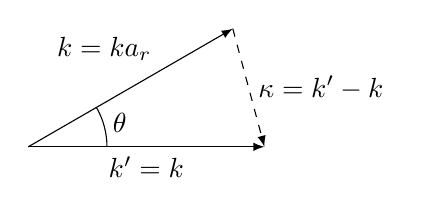
\begin{tikzpicture}
\draw[-latex] (0,0) -- (3,0) node[pos=0.5,below]{$\kvec{k}'=k\az$}coordinate(aa);
\draw[-latex] (0,0) --++ (30:3) node[pos=0.65,above left]{$\kvec{k}=k\kvec{a}_r$}coordinate(bb);
\draw[-latex,dashed] (bb)--(aa)node[pos=0.5,right]{$\kvec{\kappa}=\kvec{k}'-\kvec{k}$};
\draw([shift={(0:1)}]0,0) arc (0:30:1)node[pos=0.6,right]{$\theta$};
\end{tikzpicture}
\caption{بارن تخمین میں دو تفاعل موج: \عددی{k'} آمدی رخ جبکہ \عددی{k} بکھراو رخ ہے۔}
\label{شکل_بکھراو_آمدی_بکھراو_رخ}
\end{figure}


%=========
\ابتدا{مثال}
کم توانائی نرم کرہ بکھراو درج ذیل مخفیہ لیں 
\begin{align}
	V(r)=
	\begin{cases}
		V_0, & r\leq a \text{\RL{اگر}} \\
		0, & r>a \text{\RL{اگر}}
	\end{cases}
\end{align}
کم توانائی کی صورت میں \عددی{\theta} اور \عددی{\phi} کا غیر تابع حیطہ بکھراو درج ذیل ہوگا۔
\begin{align}
	f(\theta, \phi)\cong-\frac{m}{2\pi\hslash^2}V_0\left(\frac{4}{3}\pi a^3\right)
\end{align}
تفریقی عمودی تراش 
\begin{align}
	\frac{\dif\sigma}{\dif\Omega}=\abs{f}^2\cong\left(\frac{2mV_0a^3}{3\hslash^2}\right)^2
\end{align}
اور کل عمودی تراش درج ذیل ہوگا۔ 
\begin{align}
	\sigma\cong4\pi\left(\frac{2mV_0a^3}{3\hslash^2}\right)^2
\end{align}
\انتہا{مثال}
ایک کروی تشاکلی مخفیہ \عددی{V(r)=V(r)} کے لئے جو ضروری نہیں کہ کم توانائی پر ہو تخمین بارن دوبارہ سادہ روپ اختیار کرتا ہے۔ درج ذیل متعارف کرتے ہوئے 
\begin{align}
	\kappa\equiv k'-k
\end{align}
\عددی{r_0} تکمل کے قطبی محور کو \عددی{\kappa} پر رکھتے ہوئے درج ذیل ہوگا 
\begin{align}
	(k'-k)\cdot r_0 = \kappa r_0\cos\theta_0
\end{align}
یوں درج ذیل حاصل ہوگا
\begin{align}
	f(\theta)\cong-\frac{m}{2\pi\hslash^2}\int e^{i\kappa r_0\cos\theta_0}V(r_0)r^2_0\sin\theta_0\dif r_0\dif\theta_0\dif\phi_0
\end{align}
متغیر \عددی{\phi_0} کے لحاظ سے تکمل \عددی{2\pi} دیگا اور \عددی{\theta_0} تکمل کو ہم پہلے دیکھ چکے ہیں \حوالہء{مساوات \num{11.59}} دیکھیں۔ یوں \عددی{r} کے زیرنوشت کو نہ لکھتے ہوئے درج ذیل رہ جائے گا
\begin{align}
	f(\theta)\cong-\frac{2m}{\hslash^2\kappa}\int_{0}^{\infty}rV(r)\sin(\kappa r)\dif r، && \text{\RL{کروی تشاکل}}
\end{align}
\عددی{f} کی زاویائی تابیعت \عددی{\kappa} میں سموئی گئی ہے \حوالہء{شکل  \حوالہ{شکل_بکھراو_آمدی_بکھراو_رخ}} کو دیکھ کر درج ذیل لکھا جا سکتا ہے
\begin{align}
	\kappa = 2k\sin(\theta/2)
\end{align}
\ابتدا{مثال}
یوکاوا بکھراو۔ یوکاوا مخفیہ جو جوہری مرکزہ کے بیچ بندشی قوت کا ایک سادہ نمونہ پیش کرتا ہے کا روپ درج ذیل ہے جہاں \عددی{\beta} اور \عددی{\mu} مستقلات ہیں
\begin{align}
	V(r) = \beta\frac{e^{-\mu r}}{r}
\end{align}
تخمین بارن درج ذیل دیگا 
\begin{align}
	f(\theta)\cong-\frac{2m\beta}{\hslash^2\kappa}\int_{0}^{\infty}e^{-\mu r}\sin(\kappa r)\dif r=-\frac{2m\beta}{\hslash(\mu^2+\kappa^2)}
\end{align}
آپ کو \حوالہء{سوال \num{11.11}} میں یہ تکمل حل کرنے کو کہا گیا ہے۔
\انتہا{مثال}
\ابتدا{مثال}
ردرفورڈ بکھراو۔ مخفیہ یوکاوا میں \عددی{\beta=q_1q_2/4\pi\epsilon_0} اور \عددی{\mu=0} پُر کرنے سے مخفیہ کولمب حاصل ہوگا جو دو نقطی باروں کے بیچ برقی باہم عمل کو بیان کرتا ہے۔ ظاہر ہے کہ حیطہ بکھراو درج ذیل ہوگا 
\begin{align}
	f(\theta)\cong-\frac{2mq_1q_2}{4\pi\epsilon_0\hslash^2\kappa^2}
\end{align}
یا \حوالہء{مساوات \num{11.89} اور \num{11.51}} استعمال کرتے ہوئے درج ذیل ہوگا 
\begin{align}
	f(\theta)\cong-\frac{q_1q_2}{16\pi\epsilon_0E\sin^2(\theta/2)}
\end{align}
اس کا مربع ہمیں تفریقی عمودی تراش دیگا 
\begin{align}
	\frac{\dif\sigma}{\dif\Omega}=\left[\frac{q_1q_2}{16\pi\epsilon_0E\sin^2(\theta/2)}\right]^2
\end{align}
جو ٹھیک کلیہ ردرفورڈ \حوالہء{مساوات \num{11.11}} ہے۔ آپ دیکھ سکتے ہیں کہ کولمب مخفیہ کے لئے کالسیکی میکانیات تخمین بارن اور کوانٹائی نظریہ میدان تمام ایک  جیسا نتیجہ دیتے ہیں۔ ہم کہہ سکتے ہیں کہ کلیہ ردرفورڈ ایک مضبوط کلیہ ہے۔
\انتہا{مثال}
\ابتدا{سوال}
اختیاری توانائی کے لئے نرم کرہ بکھراو کا حیطہ بکھراو بارن تخمین سے حاصل کریں دکھائیں کہ کم توانائی حد میں اس سے \حوالہء{مساوات \num{11.82}} حاصل ہوگا۔
\انتہا{سوال}
\ابتدا{سوال}
\حوالہء{مساوات \num{11.91}} میں تکمل کی قیمت تلاش  کر کے دائیں ہاتھ ریاضی فقرہ  کی تصدیق کریں۔
\انتہا{سوال}
\ابتدا{سوال}
بارن تخمین میں یوکاوا مخفیہ سے بکھراو کا کل عمودی تراش تلاش کریں۔ اپنے جواب کو \عددی{E} کا تفاعل لکھیں۔
\انتہا{سوال}
\ابتدا{سوال}
درج ذیل اقدام \حوالہء{سوال \num{11.4}} کے مخفیہ کے لئے کریں۔

(الف) کم توانائی تخمین بارن میں \عددی{f(\theta, D(\theta))} اور \عددی{\sigma} کا حساب لگائیں۔

(ب) تخمین بارن میں اختیاری توانائیوں کے لئے \عددی{f(\theta)} کا حساب لگائیں۔

(ج) دکھائیں کہ آپ کے نتائج مناسب خطوں میں \حوالہء{سوال \num11.4} کے جواب کے مطابق ہیں۔
\انتہا{سوال}

%=================================

\جزوحصہ{تسلسل بارن}
تخمین بارن روح کے لحاظ سے کلاسیکی نظریہ بکھراو میں تخمین ضرب کی طرح ہے۔ ایک ذرہ کو منتقل عرضی ضرب کا حساب کرنے کے لئے ہم تخمین ضرب میں فرض کرتے ہیں
 کہ ذرہ ایک سیدھی لیکر پر ہی چلے جاتا ہے  (شکل \حوالہ{شکل_بکھراو_تخمین_ضرب})۔  ایسی صورت میں درج ذیل ہوگا
\begin{align}
	I=\int F_\perp\dif t
\end{align}
%
\begin{figure}
\centering
\begin{tikzpicture}
\pgfmathsetmacro{\ang}{atan(1/2.5)}
\draw[] (0,0) -- (6,0) node[pos=0.55, circle, inner sep=1.5pt,fill=black]{} node[pos=0.55, below]{\RL{نقطہ بکھراو}} ;
\draw[dashed] (0,1) -- (6,1) node[pos=0.5, circle, inner sep=1.5pt,fill=black]{};
\draw[thick,-stealth] (0,1) to [out=0,in=-160] (6,2) node[above]{\RL{اصل خط حرکت}};
\draw[-stealth] (3,1) -- (3,2) node[above]{$F_{\perp}$}; 
\draw[dashed] (3.5,1) -- (6,2);
\draw[] ([shift={(0:1)}]3.5,1) arc (0:\ang:1) node[pos=0.6,right]{$\theta$};
\draw[stealth-stealth] (0.25,0) --++ (0,1) node[pos=0.5,left]{$b$};
\end{tikzpicture}
\caption{ ذرہ  کو منتقل معیار حرکت کا حساب کرتے ہوئے،تخمین ضرب کی ترکیب  میں فرض کیا  جاتا ہے کہ ذرہ بغیر  مڑے سیدھی لکیر پر حرکت کیے جاتا ہے۔}
\label{شکل_بکھراو_تخمین_ضرب}
\end{figure}

اگر ذرہ زیادہ نہیں مڑے تب یہ ذرہ کو منتقل معیار حرکت کی ایک اچھی تخمین ہوگی اور یوں زاویہ بکھراو درج ذیل ہوگا جہاں \عددی{p} آمدی معیار حرکت ہے 
\begin{align}
	\theta\cong\tan^{-1}(I/p)
\end{align}
اسے ہم رتبہ اول تخمین ضرب کہہ سکتے ہیں نہ مڑنے کی صورت کو صفر رتبی کہا جائے گا اسی طرح صفر رتبی تخمین بارن میں آمدی مستوی موج بغیر کسی تبدیلی کے گزرے گی اور ہم نے جو کچھ گزشتہ حصہ میں دیکھا وہ در حقیقت اس کی رتبہ اول تصحیح ہے۔ ہم توقع کر سکتے ہیں کہ اسی تصور کو بار بار استعمال کرتے ہوئے ہم زیادہ بلند رتبی تصحیح کا ایک تسلسل پیدا کر کے بالکل  ٹھیک جواب پر مرکوز ہو سکتے ہیں۔

مساوات شروڈنگر کی تکملی روپ درج ذیل ہے
\begin{align}
	\psi(r)=\psi_0(r)+\int g(r-r_0)V(r_0)\psi(r_0)\dif^3r_0
\end{align}
جہاں \عددی{\psi_0} آمدی موج ہے
\begin{align}
	g(r)\equiv-\frac{m}{2\pi\hslash^2}\frac{e^{ikr}}{r}
\end{align}
تفاعل گرین ہے۔ جس میں میں نے اپنی آسانی کے لئے جزو ضربی \عددی{2m/\hslash^2} شامل کیا ہے اور \عددی{V} مخفیہ بکھراو ہے۔ اس کو درج ذیل دیکھا جا سکتا ہے
\begin{align}
	\psi = \psi_0+\int gV\psi
\end{align}
فرض کریں ہم \عددی{\psi} کی اس ریاضی جملہ کو لیکر اسے تکمل کی علامت کے اندر لکھیں 
\begin{align}
	\psi=\psi_0+\int gV\psi_0+\iint gVgV\psi
\end{align}
اس عمل کہ بار بار دوہرانے سے ہمیں \عددی{\psi} کا ایک تسلسل حاصل ہوگا
\begin{align}\label{مساوات_بکھراو_بارن_تخمین_تسلسل}
	\psi=\psi_0+\int gV\psi_0+\iint gVgV\psi_0+\iiint gVgVgV\psi_0+\dots
\end{align}
ہر متکمل میں آمدی تفاعل موج \عددی{\psi_0} کے علاوہ \عددی{gV} کے مزید زیادہ طاقتیں پائی جاتی ہیں۔ بارن کی تخمین اول اس تسلسل کو دوسرے جزو کے بعد ختم کرتا ہے تاہم آپ دیکھ سکتے ہیں کہ بلند رتبی تصحیح کس طرح پیدا کی جائیں گی۔
\begin{figure}
\centering
\begin{tikzpicture}
\pgfmathsetmacro{\a}{1.25}
\pgfmathsetmacro{\r}{0.75}
\pgfmathsetmacro{\d}{0.25}
\draw[->-=0.6] (0,0) node[left]{$\psi=$} --++ (\a,0) node[pos=0.5,below]{$\psi_0$};
\draw[] (\a +\d,0) node[]{$+$};
\draw[->-=0.25] (\a+2*\d,0) --++ (\a,0) node[pos=0.25,below]{$\psi_0$} coordinate(aa);
\draw[] (aa) node[circle, inner sep= 1.5pt, fill=black]{} node[below]{$V$} circle (\r);
\draw[] (aa) --++ (30:1.25) node[pos=0.25,shift={(-60:0.5em)}]{$g$};
\draw[] (2*\a +4*\d+\r,0) node[]{$+$};
\draw[->-=0.3] (2*\a +5*\d+\r,0) --++ (\a,0) node[pos=0.3,below,xshift=-0.1em]{$\psi_0$} coordinate(aa);
\draw[] (aa) node[circle, inner sep= 1.5pt, fill=black]{} node[below]{$V$} circle (\r);
\draw[] (aa) --++ (20:0.5) node[pos=0.5,shift={(110:0.5em)}]{$g$} node[circle, inner sep=1.5pt,fill=black]{} node[below]{$V$} --++ (80:1) node[pos=0.5,right]{$g$};
\draw[] (3*\a +6*\d+2*\r,0) node[]{$+$};
\draw[->-=0.3] (3*\a +7*\d+2*\r,0) --++ (0.75*\a,0) node[pos=0.3,below,xshift=-0.1em]{$\psi_0$} node[circle, inner sep= 1.5pt, fill=black]{} node[above]{$V$}coordinate(bb); 
\draw[] (4*\a +7*\d+2*\r,0) coordinate(aa) circle (\r);
\draw[] (bb) --++ (-40:0.5) node[pos=0.5,shift={(-130:0.5em)}]{$g$} node[circle, inner sep=1.5pt,fill=black]{} node[below]{$V$} --++ (45:0.75) node[pos=0.5,shift={(-45:0.5em)}]{$g$}node[circle, inner sep=1.5pt,fill=black]{}node[above left]{$V$}--++(-10:1)node[pos=0.75,above]{$g$};
\draw[] (5*\a +7*\d+3*\r,0) node[]{$+\cdots$};
\end{tikzpicture}
\caption{بارن تسلسل (مساوات \حوالہ{مساوات_بکھراو_بارن_تخمین_تسلسل}) کا  نظیری مفہوم۔}
\label{شکل_بکھراو_نظیری_مفہوم}
\end{figure}

بارن تسلسل کا خاکہ شکل \حوالہ{شکل_بکھراو_نظیری_مفہوم}  میں پیش کیا گیا ہے۔ صفر رتبی \عددی{\psi} پر مخفیہ کا کوئی اثر نہیں ہوگا رتبی اول میں اسے ایک چوٹ پڑتی ہے جس کے بعد یہ کسی نئے رخ چلے جائے گا۔ دوم رتبی میں اسے ایک چوٹ پڑتی ہے جس کے بعد یہ ایک نئے مقام پر پہنچتا ہے جہاں اسے دوبارہ ایک چوٹ پڑتی ہے جس کے بعد یہ ایک نئے راہ پر چل نکلتا ہے وغیرہ وغیرہ۔ اسی کے بنا پر بعض اوقات تفاعل گرین کو اشاعت کار کہا جاتا ہے جو ایک باہم عمل اور سورے کے بیچ خلل کی اشاعت کس طرح ہوتی ہے۔ تسلسل بارن اضافیتی کوانٹائی میکانیات کی فینمن تشریح کا سبب بنا جس میں اشکال فینمن میں جزو ضربی راس \عددی{V} اور اشاعت کار \عددی{g} کو ایک   ساتھ جوڑ کر سب کچھ بیان کیا جاتا ہے۔

\ابتدا{سوال}
تخمین ضرب میں ردرفورڈ بکھراو کے لئے \عددی{\theta} کو ٹکراؤ مقدار معلوم کا تفاعل تلاش کریں۔ دکھائیں کہ مناسب حدوں کے اندر آپ کا نتیجہ بالکل  ٹھیک ریاضی فقرہ \حوالہء{سوال \num{11.1} (الف)} کے مطابق ہے۔
\انتہا{سوال}
\ابتدا{سوال}
بارن کی دوسری تخمین میں کم توانائی نرم کرہ بکھراو کے لئے حیطہ بکھراو تلاش کریں۔

جواب: \عددی{-(2mV_0a^3/3\hslash^2)[1-(4mV_0a^2/5\hslash^2)]}
\انتہا{سوال}
\ابتدا{سوال}
یک بُعدی مساوات شروڈنگر کے لئے تفاعل گرین تلاش کر کے \حوالہء{مساوات \num{11.67}} کا مماثل تکملی روپ تیار کریں۔

جواب:
\begin{align}
	\psi(x)=\psi_0(x)-\frac{im}{\hslash^2k}\int_{-\infty}^{\infty}e^{ik\abs{x-x_0}}V(x_0)\psi(x_0)\dif x_0
\end{align}
\انتہا{سوال}
\ابتدا{سوال}
مبدا پر بغیر اینٹوں کی دیوار کی صورت میں وقفہ \عددی{-\infty<x<\infty} پر یک بُعدی بکھراو کے لئے \حوالہء{سوال \num{11.16}} کا نتیجہ استعمال کرتے ہوئے تخمین بارن تیار کریں۔ یعنی \عددی{\psi(x_0)\cong\psi_0(x_0)} تصور کرتے ہوئے \عددی{\psi_0(x)=Ae^{ikx}} منتخب کر کے تکمل کی قیمت تلاش کریں۔ دکھائیں کہ انعکاسی عددی سر درج ذیل روپ اختیار کرتا ہے
\begin{align}
	R\cong\left(\frac{m}{\hslash^2k}\right)^2\abs{\int_{-\infty}^{\infty}e^{2ikx}V(x)\dif x}^2
\end{align}
\انتہا{سوال}
\ابتدا{سوال}
ایک ڈیلٹا تفاعل \حوالہء{مساوات \num{2.114}} اور ایک متناہی چوکور کنواں \حوالہء{مساوات \num{2.145}} سے بکھراو کے لئے تفصیلی عددی سر \عددی{(T = 1 - R)} کو یک بُعدی تخمین بارن \حوالہء{سوال \num{11.17}} کی مدد سے حاصل کریں۔ اپنے جوابات کا بالکل  ٹھیک جوابات \حوالہء{مساوات \num{2.141} اور \num{2.169}} کے ساتھ موازنہ کریں۔
\انتہا{سوال}
\ابتدا{سوال}
آگے رخ حیطہ بکھراو کے خیالی جزو اور کل عمودی تراش کے بیچ رشتہ دینے والا مسئلہ بصریات ثابت کریں 
\begin{align}
	\sigma = \frac{4\pi}{k}Im(f(0))
\end{align}
اشارہ: \حوالہء{مساوات \num{11.47} اور \num{11.48}} استعمال کریں۔
\انتہا{سوال}
\ابتدا{سوال}
Missing Question
\begin{align}
	V(r) = Ae^{-\mu r^2}
\end{align}
\انتہا{سوال}

